% !TeX program = xelatex
% =====================================================================
% 2026 高教社杯 C 题 · 修正版论文
% 相对原稿（数模.tex）的修正见 README 同目录的《论文问题清单》
% 本文件修正内容：补全问题三/问题四/模型评价/参考文献/附录；
% 统一符号体系；修正 η、pi_t、表格列数、重复 label、硬编码编号；
% 全部数值与程序输出（result*.xlsx、*_结果汇总.txt）逐项核对。
% =====================================================================
\documentclass{cumcmthesis}
\usepackage[framemethod=TikZ]{mdframed}
\usepackage{graphicx}
\usepackage{adjustbox}
\usepackage{url}
\usepackage{subcaption}
\usepackage{booktabs}
\usepackage{multirow}
\usepackage{amsmath,amssymb}
\usepackage{listings}

% 让所有浮动体（表格/图）内容统一用小一号字，控制篇幅
\makeatletter
\g@addto@macro\@floatboxreset{\small}
\makeatother

\title{基于线性规划对微网与外网电力调控策略的研究}
\tihao{C}
\baominghao{121}
\schoolname{上海交通大学}
\membera{张航}
\memberb{刘允禾}
\memberc{高慧鑫}
\supervisor{高晓沨}
\yearinput{2026}
\monthinput{09}
\dayinput{13}

\begin{document}

\maketitle

\begin{abstract}
    随着“双碳”目标的推进和微网系统的快速发展，微网的经济调度成为促进新能源就地消纳、降低用能成本的关键。本文在分时电价机制下，基于给定的电价、小区负载、光伏发电功率数据，建立数学模型，协调外网购电与储能充放电，实现购电费用最小化。全文统一采用 10 分钟为一个时段（$\Delta t=1/6$ h，每天 $T=144$ 个时段），储能效率 $\eta=0.9$、容量 12000 kWh（安全区间 1200$\sim$10800 kWh）、最大充放电功率 5000 kW。\newline \hspace*{2em}
    针对问题一，全部输入数据已知，该问题为确定性优化问题。以全天购电费用最小为目标，结合功率平衡、储能状态转移、SOC 安全区间、始末电量守恒、充放电功率互斥、非负性等 6 类约束，建立\textbf{混合整数线性规划（MILP）模型}。求解得到全天总购电量为\textbf{59\,482.6990 kWh}，全天总购电费为\textbf{35\,126.9486 元}；平均购电单价 0.5906 元/kWh，显著低于电价均值 0.7662 元/kWh，说明储能成功实现了“谷充峰放”套利。本文进一步证明充放电互斥的 0-1 变量在 $\eta<1$ 时可松弛为连续变量：实测 LP 松弛与 MILP 最优值完全相同（差为 0），为后续两问采用纯 LP 提供了依据。\newline \hspace*{2em}
    针对问题二，负载与光伏均需预测。先对负载做周期性检验：其日总量自相关在滞后 7 天处出现孤立峰值 0.988（滞后 1 天仅 0.374），故负载采用\textbf{“上周同一天”}预测；光伏无周周期特征（滞后 7 天仅 0.929），改用\textbf{“前 3 天滑动平均”}（其全年 MAE 154.5 kW，优于“前 1 天”的 185.3 kW）。再以\textbf{报童模型}确定安全裕量：多买 1 kWh 成本 $\pi_t$、少买 1 kWh 需按 $5\pi_t$ 紧急购电，故临界分位数 $\alpha^*=4/5=0.80$。建立\textbf{两阶段线性规划模型}（日前 LP + 逐槽实时平衡），并采用逐时段滚动分位数裕量。全年（2025-02-01 起 334 天）总购电费为\textbf{13\,949\,108.5 元}，其中计划购电量 21\,442\,248.8 kWh、紧急购电量 141\,988.6 kWh（占 0.66\%）。\newline \hspace*{2em}
    针对问题三，引入 0:00、6:00、12:00、18:00 四阶段滚动调整与双向偏差惩罚（下调违约按 $0.5\pi_t$、上调超出按 $1.5\pi_t$）。报童模型在两阶段给出不同临界分位（计划阶段 0.80、调整阶段 0.70），故统一裕量取区间中点 $\alpha^*=0.75$。关键工作是证明“逐槽被动平衡规则”可用四组上界约束被 LP \textbf{精确嵌入}（无需“LP+仿真”嵌套迭代），并通过逐时段对比验证 LP 最优解物理可执行。全年总购电费为\textbf{13\,589\,362.4 元}，较问题二降低 35.97 万元（2.58\%）；本文另给出\textbf{完美信息下界 12\,254\,765.7 元}，据此量化预报误差的代价为 133.5 万元（9.82\%）。\newline \hspace*{2em}
    针对问题四，改用附件 4 的逐日波动电价重算问题二与问题三。全年费用分别为\textbf{14\,634\,080.5 元}（+4.91\%）与\textbf{14\,210\,954.8 元}（+4.57\%）。受控分解表明，涨价并非源于日内峰谷比升高（窗口均价反而由 0.7662 降至 0.7575），\textbf{97.2\%} 的增量来自\textbf{逐日电价漂移}：日购电量与当日电价水平的相关系数达 $+0.9651$，即“高负载日恰为高电价日”，而储能容量远不足以跨日套利。\newline \hspace*{2em}
    本文最后给出灵敏度与稳健性分析、模型的评价与推广。所有结果均由 \texttt{run\_all.py} 一键复现，数值与图表见交付文件 \texttt{result1\~{}4*.xlsx}。
    \keywords{线性规划\quad 报童模型\quad 滚动优化\quad 微网经济调度\quad 灵敏度分析}
\end{abstract}

\section{问题重述}
\subsection{问题背景}
随着“碳达峰、碳中和”目标的推进，以光伏为代表的分布式能源正经历跨越式发展。微网能缓解大规模并网带来的反向潮流、电压波动等问题，成为新型电力系统的重要形态。而外网普遍实行峰谷分时电价机制，电价在不同时段差异显著。为满足小区负载并降低微网购电费用，制定合理的购电策略与储能充放电计划尤为重要。

\subsection{数据说明}
题目提供四份附件，本文对其口径作如下统一定义（时间标签均取区间的\textbf{右端点}，即“0:10”表示区间 $[0{:}00,0{:}10)$）：

\begin{center}
\small
\begin{tabular}{clc}
\hline
附件 & 内容 & 时间跨度 \\
\hline
附件 1 & 基准日电价（元/kWh）、小区负载（kW）、光伏发电预测功率（kW），各 144 点 & 1 天 \\
附件 2 & 全年小区负载（kW）与光伏实际发电功率（kW），$365\times144$ & 全年 \\
附件 3 & 全年光伏发电功率预报：每天 0:00、6:00、12:00、18:00 各发布一次， & 全年 \\
       & 每次给出未来 24 个小时的\textbf{整点}（24 点）预报 & \\
附件 4 & 全年逐日逐时段实时电价（元/kWh），$365\times144$ & 全年 \\
\hline
\end{tabular}
\end{center}

其中附件 3 的“预报 $k$ 小时”为发布后第 $k$ 个整点时刻的\textbf{瞬时功率}（点值），本文按整点线性插值到 10 分钟时段；若误按“小时平均功率”处理，全年 MAE 将由 191.7 kW 恶化到 361.6 kW。四份附件的范围核验见 \texttt{数据概览.txt}。

\subsection{需要解决的问题}
\noindent\textbf{问题一：}假设每天电价与小区负载固定、光伏发电功率预测已知，要求微网提供的电能不低于小区负载、且储能设备在 0:00 与 24:00 的储电量相同，给出当天 0:00 制定计划购电策略的数学模型，并给出题目指定时间段的购电量、全天购电量与购电费。

\noindent\textbf{问题二：}每天电价仍取附件 1 的固定分时电价，但小区负载与光伏发电功率逐日逐时段波动且事先未知。若实际供电量低于小区负载，需以 5 倍实时电价紧急购电；常规时段购电按计划购电量计费。给出每天 0:00 制定计划购电策略的数学模型。

\noindent\textbf{问题三：}每天 0:00、6:00、12:00、18:00 可获得未来 24 小时整点的光伏发电功率预报，允许滚动调整购电策略。计划购电量高于调整购电量的部分，违约电价为其 50\%；调整购电量高于计划购电量的部分，超出部分按 1.5 倍电价支付。总购电费用包括计划购电费用、紧急购电费用与调整购电量的相关费用，要求建立当天购电策略的数学模型。

\noindent\textbf{问题四：}外网电价实时波动（附件 4），重新建立微网当天购电策略的数学模型，并与问题二、问题三的结果对比。

\section{问题分析}
\subsection{问题一的分析}
问题一的全部输入（电价、负载、光伏）均为已知常量，故为确定性优化问题。由于购电费用与各决策量线性相关、约束均可写成线性等式或不等式，可建立线性规划模型并用单纯形/分支定界法求得全局最优。特别地，储能“充放电互斥”这一逻辑约束通常需要引入 0-1 变量；但本文证明：当储能往返效率 $\eta^2<1$ 时，同时充放电会白白损失 $(1-\eta^2)$ 比例的能量，最优解中必然不会出现 $c_t\cdot d_t>0$，故该 0-1 变量可松弛为连续变量。我们同时用 MILP 与 LP 求解并比对，两者最优值完全相同，见 6.4 节。

\begin{figure}[htbp]
\centering
\begin{minipage}[c]{0.44\textwidth}
    \centering
    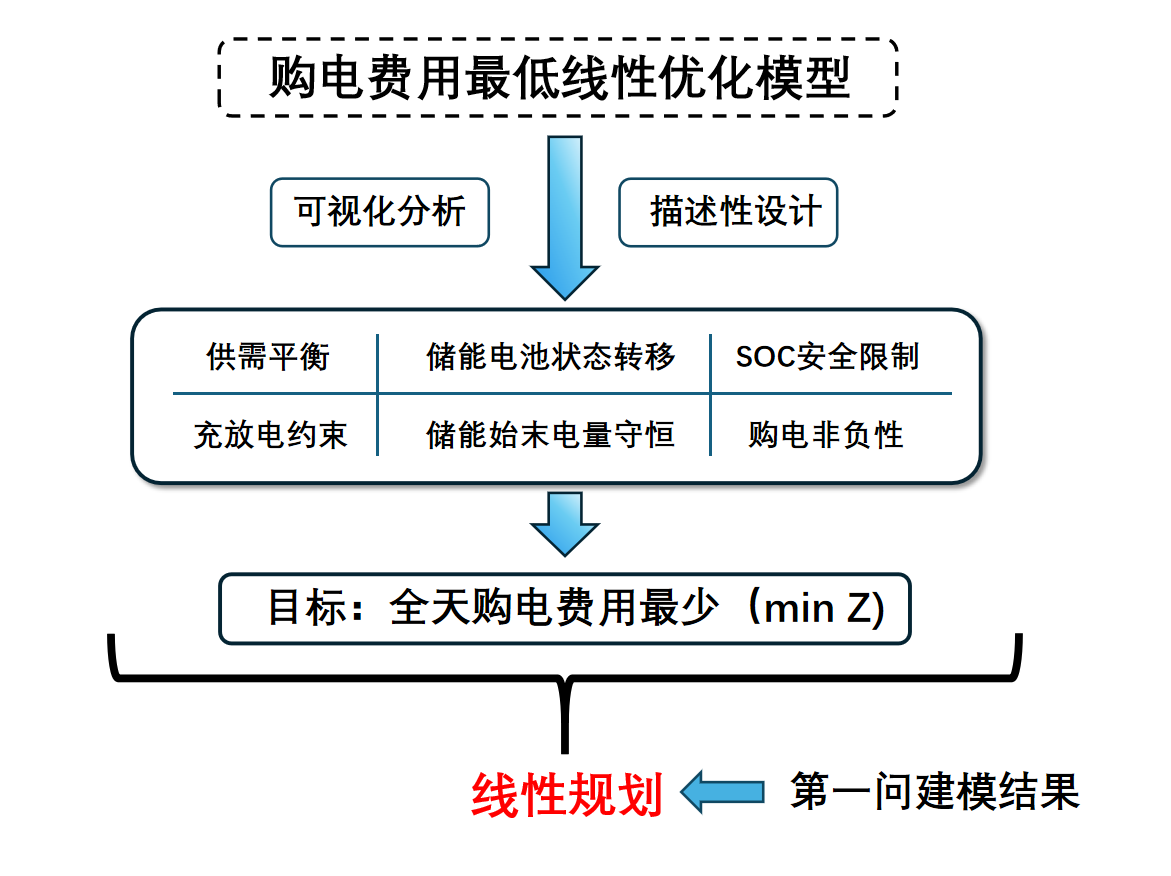
\includegraphics[width=0.95\textwidth]{第一问思维框架.png}
    \subcaption{问题一思维框架}
\end{minipage} \hfill
\begin{minipage}[c]{0.48\textwidth}
    \centering
    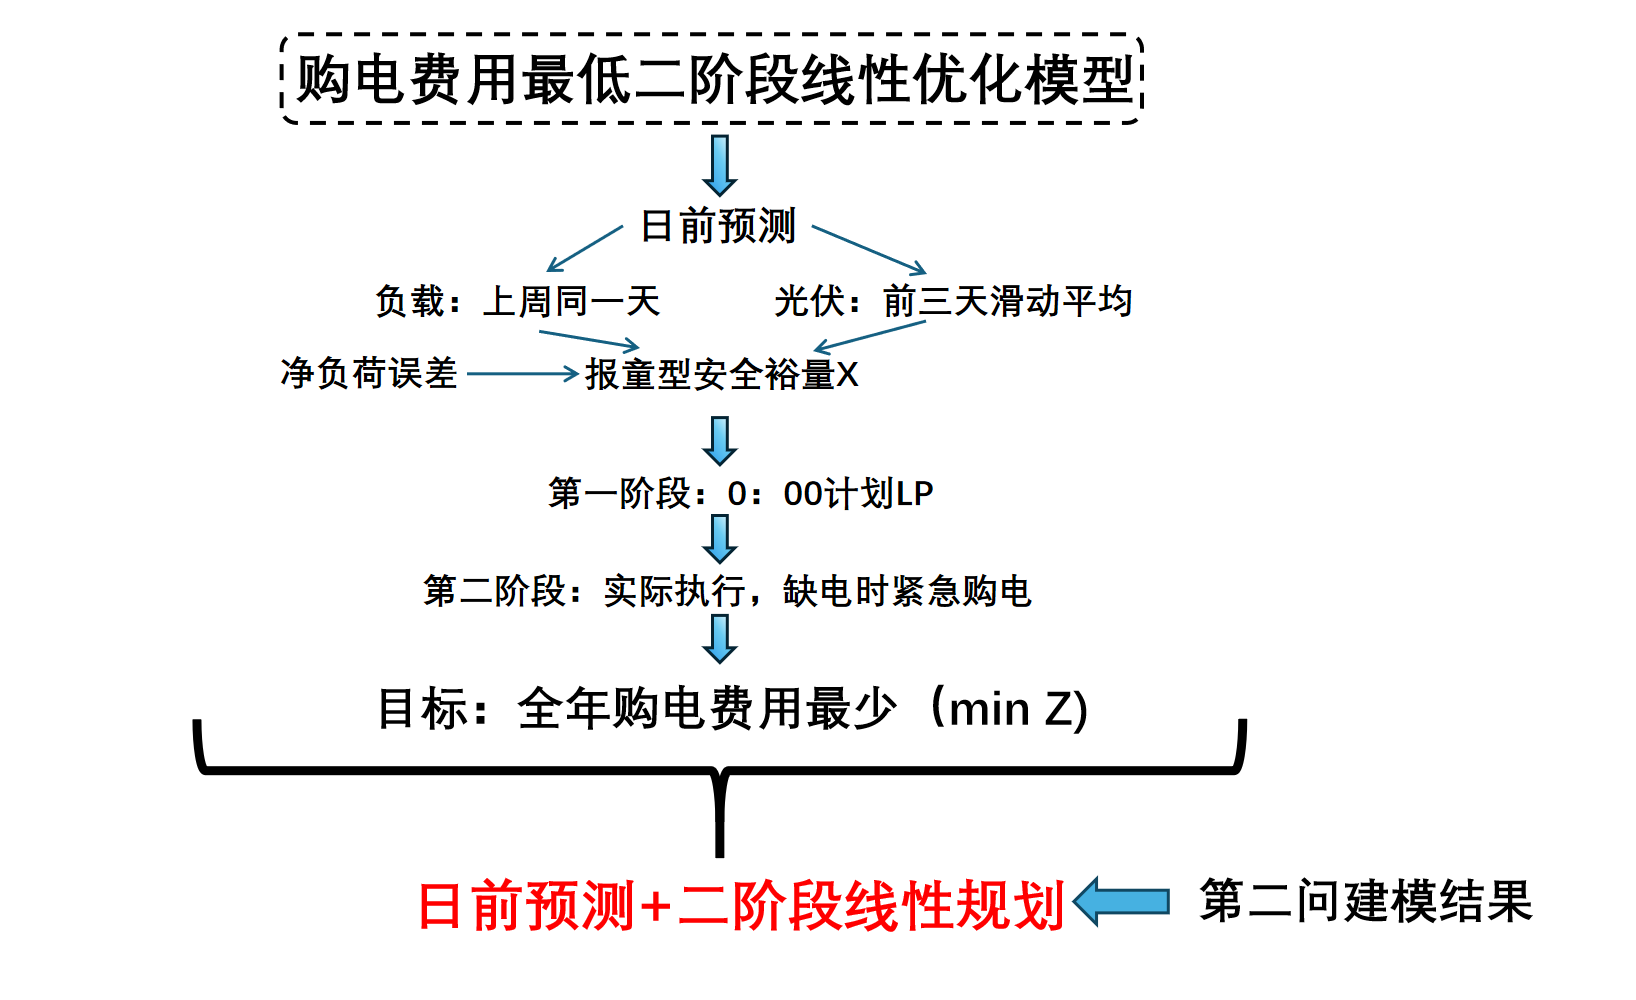
\includegraphics[width=1\textwidth]{第二问思维导图.png}
    \subcaption{问题二思维框架}
\end{minipage}
\caption{问题一与问题二的思维框架}
\end{figure}

\subsection{问题二的分析}
问题二的难点由“优化”转为“优化 + 不确定性”。计划购电量在 0:00 锁定后不可更改，当实际净负荷高于计划时，缺口只能以 5 倍电价紧急购电；而多买 1 kWh 仅损失 1 倍电价的资金成本。二者的不对称性正是\textbf{报童模型}的适用场景：以历史预测误差的分布为“需求分布”，取临界分位数为安全裕量即可最小化期望费用。因此本文采用“日前 LP（含报童裕量）+ 逐槽实时平衡”的两阶段结构：第一阶段决定买多少，第二阶段决定储能如何实时平衡。

\subsection{问题三的分析}
问题三在问题二基础上增加了两层信息：一是光伏预报在一天内多次更新，二是“改了计划要罚钱”。调整阶段两侧的边际成本变为“多买 $1.5\pi_t$”与“少买（退回 $0.5\pi_t$ 后仍需按 $5\pi_t$ 补）”之比，故其临界分位与计划阶段不同。同时，储能的实际动作由“逐槽被动平衡”规则决定，若在 LP 中近似处理，可能出现“LP 认为最优、物理上执行不了”的解。因此本文的核心工作是：\textbf{把逐槽规则精确嵌入 LP}，并给出等价性验证。

\begin{figure}[htbp]
\centering
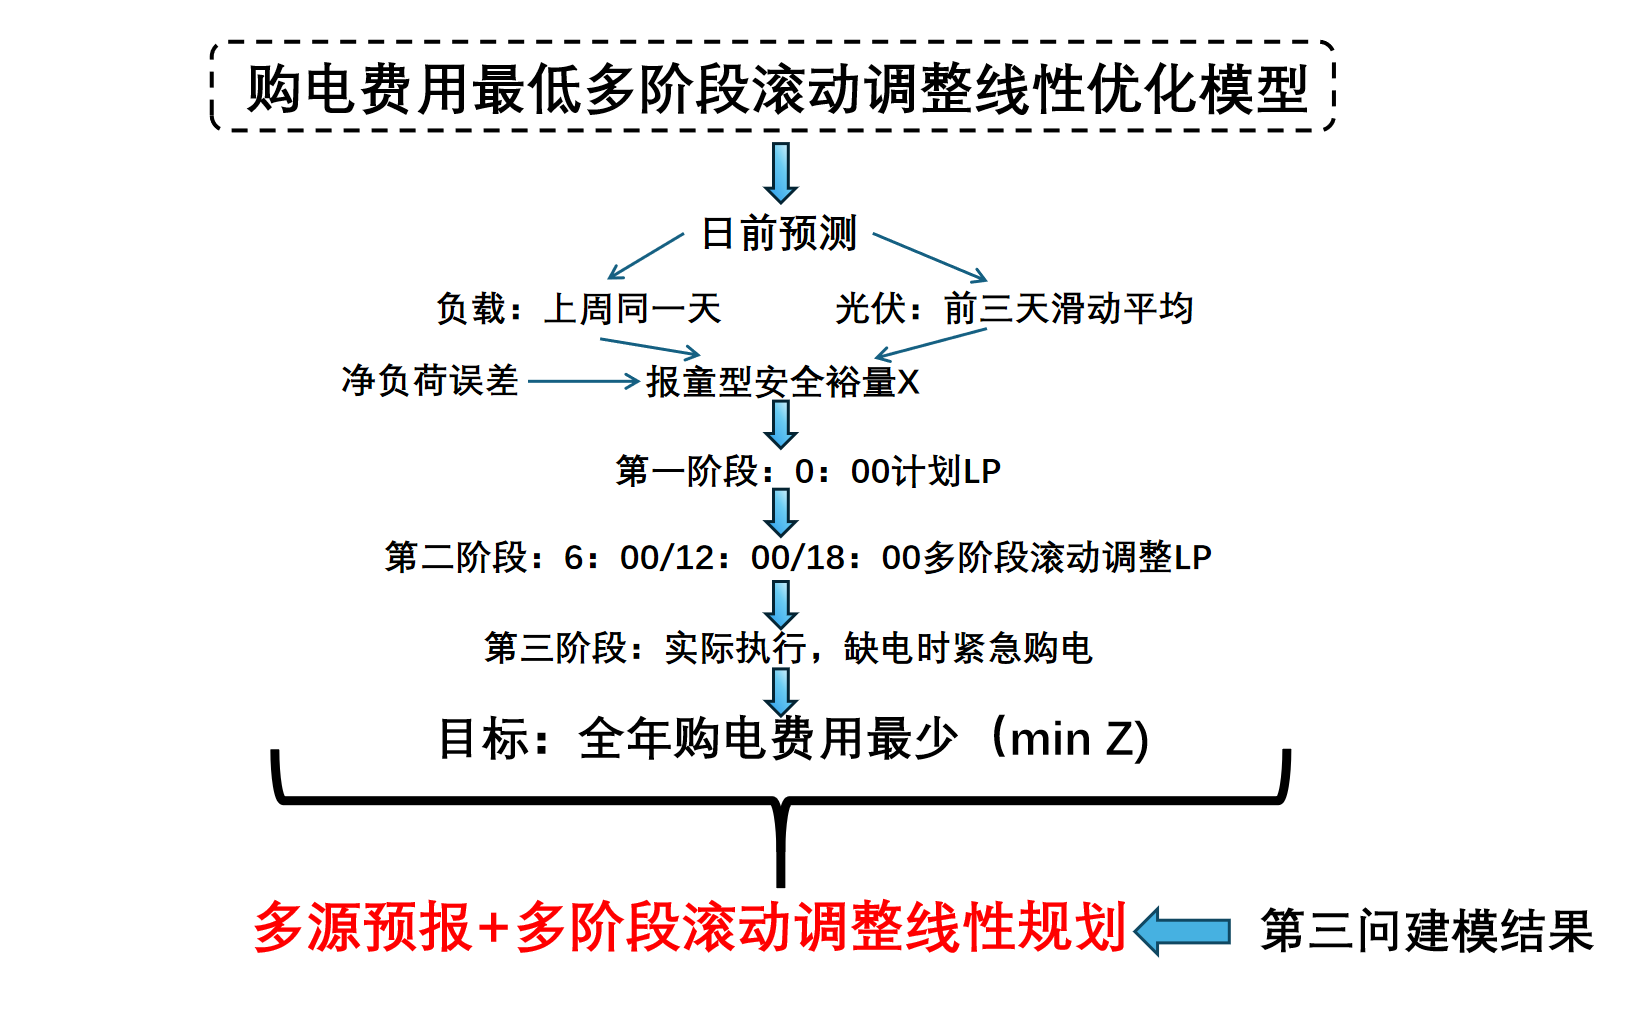
\includegraphics[width=.62\textwidth]{问题三思维导图.png}
\caption{问题三思维框架}
\end{figure}

\subsection{问题四的分析}
问题四将固定电价替换为附件 4 的波动电价。由于电价曲线在日前市场提前公布，0:00 即可获知当天全部 144 个时段的价格，故电价无需预测，模型结构与问题二、问题三完全一致，只是目标函数中的 $\pi_t$ 由“一条日内曲线重复 365 天”变为“每天都不同”。这提供了一个天然的受控实验：\textbf{同一模型、同一预测、仅换电价}，从而可把费用变化完整归因于电价本身。

\section{模型假设}
\begin{enumerate}
    \item 微网只向外网单向购电，不考虑向电网售电，购电量非负。
    \item 储能充放电存在往返效率损失，充、放电效率均为 $\eta=0.9$；弃光不产生额外能量损耗。
    \item 储能容量 12000 kWh，荷电安全区间 $[1200,10800]$ kWh，最大充放电功率 5000 kW。
    \item 储能 0:00 储电量为 6000 kWh；问题一要求 24:00 储电量与之相同（$E_0=E_T$），问题二至问题四逐日连续（当天 24:00 的储电量顺延为次日 0:00 的初值）。
    \item 储能充放电互斥。由 $\eta^2=0.81<1$，该约束在最优解中自动满足（见 6.4 节证明与数值验证）。
    \item 紧急购电只在“储能放电与计划购电均不足以覆盖实际净负荷”时发生，其价格恒为当时段实时电价的 5 倍；计划购电与调整购电均按相应时段电价结算。
    \item 仅在 0:00 制定计划时只能使用历史数据（1 至 $d-1$ 天），当天数据未知；预测误差为随机变量，其分布由历史样本估计。
    \item 微网规模足够小，其购电行为不影响外网电价；电价曲线外生给定。
    \item 不考虑线路损耗与网络约束，购电功率不设上限（题目未给出联络线容量限制）。
\end{enumerate}

\section{符号说明}
\begin{center}
\begin{tabular}{cl}
\hline
符号 & 意义 \\
\hline
$t=1,\dots,144$ & 时段索引，$\Delta t=1/6$ h \\
$\pi_t$ & 第 $t$ 时段的外网电价（元/kWh） \\
$L_t^{\mathrm{real}},\ G_t^{\mathrm{real}}$ & 第 $t$ 时段的实际小区负载、实际光伏功率（kW） \\
$\hat L_{d,t},\ \hat G_{d,t}$ & 第 $d$ 天第 $t$ 时段的负载、光伏预测值（kW） \\
$b_t^{p},\ b_t^{a}$ & 计划购电量、调整后购电量（kW）；对应时段电量 $b_t\Delta t$（kWh） \\
$c_t,\ d_t$ & 储能充电、放电功率（kW） \\
$s_t$ & 弃光功率（kW） \\
$e_t$ & 紧急购电功率（kW） \\
$E_t$ & 第 $t$ 时段末储能电量（kWh） \\
$u_t\in\{0,1\}$ & 充放电状态指示变量（仅问题一显式使用） \\
$\delta_t^{+},\delta_t^{-}$ & 调整量相对计划的正、负偏差（kW） \\
$\eta$ & 储能充放电效率，$0.9$ \\
$P_{\max}$ & 最大充放电功率，5000 kW \\
$E_{\min},E_{\max},E_0$ & SOC 下限、上限与初值，1200 / 10800 / 6000 kWh \\
$\varepsilon_{d,t}$ & 预测误差（实际 $-$ 预报，kW）；MAE 与报童裕量共用 \\
$X_{d,t}$ & 安全裕量（kW） \\
$\tilde L_{d,t}$ & 等效预测负载（kW），$\tilde L=\hat L+X$ \\
$\alpha^{*}$ & 报童临界分位数 \\
$W$ & 裕量回看窗口（天） \\
$k_w$ & 光伏滑窗天数（前 $k_w$ 天滑动平均的回看天数） \\
\hline
\end{tabular}
\end{center}

\noindent 说明：$e_t$ 专指\textbf{紧急购电功率}，与预测误差 $\varepsilon_{d,t}$ 是两个不同的量，全文不混用。
另外，“预报 $k$ 小时”（$k=1,\dots,24$）是题面用语，指附件 3 发布后第 $k$ 个整点；它与本文的光伏滑窗天数 $k_w$ 无关，后文一律用 $k_w$ 以免混淆。

\section{数据预处理与口径说明}
\subsection{时间口径与统计窗口}
所有附件的时间标签取区间右端点，“0:10”对应区间 $[0{:}00,0{:}10)$，“0:00+1”对应 $[23{:}50,24{:}00)$。需要说明的是，题目所给 \texttt{result1.xlsx} 模板的时间标签列相对该约定整体偏移一格（首行为“0:10-0:20”、末行为“0:00+1-0:10+1”），本文按\textbf{行序}对应区间 $[10(t-1),10t)$ 填表，即模板第 2 行对应 $[0{:}00,0{:}10)$。
统计窗口统一取 \textbf{2025-02-01 至 2025-12-31 共 334 天}：前 31 天用于构造滚动预测与裕量的历史样本（预热期），不计入费用统计，避免“起算日数据不可得”的争议。

\subsection{电价、负载、光伏的日内特征}
\begin{figure}[htbp]
\centering
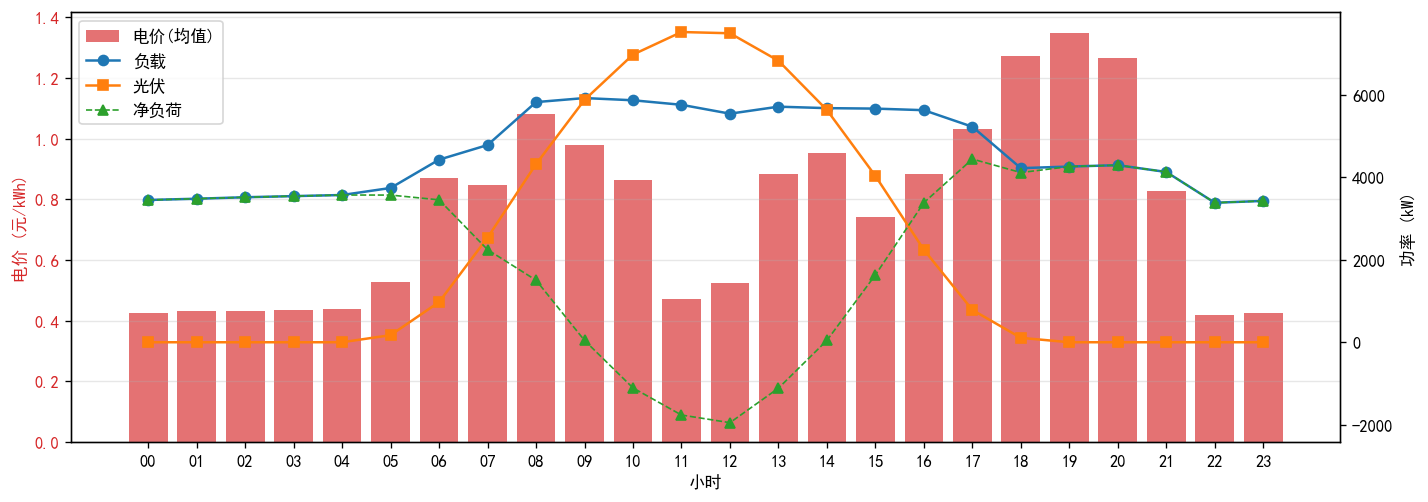
\includegraphics[width=0.62\textwidth]{逐小时.png}
\caption{电价、小区负载、光伏发电预测功率的日内变化（附件 1 逐小时均值）}
\end{figure}

如图可见：电价呈典型峰谷分时特征，范围为 $0.3713\sim1.3952$ 元/kWh、均值 0.7662 元/kWh、日内峰谷比 3.76，为储能套利提供了经济空间；小区负载呈早晚双峰，且晚高峰与电价峰段重合，是购电成本的主要来源；光伏仅在日间（约 6:00$\sim$18:00）出力、正午达峰，与电价晚高峰存在明显时间错位。若不计储能，直接按净负荷购电，全年需 16\,407\,319.6 元（附件 1 口径），这构成衡量储能价值的基准。

\begin{figure}[htbp]
\centering
\begin{minipage}[c]{0.52\textwidth}
    \centering
    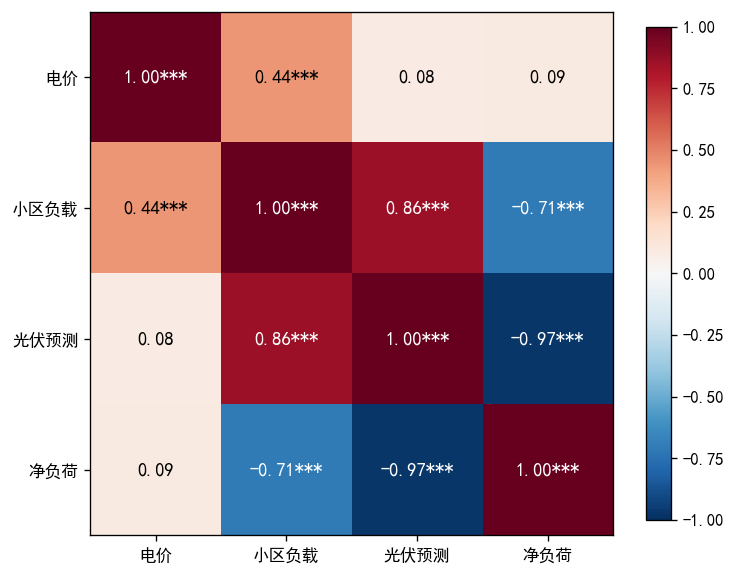
\includegraphics[width=\textwidth]{热力图.png}
    \subcaption{相关性热力图}
\end{minipage} \hfill
\begin{minipage}[c]{0.44\textwidth}
    \centering
    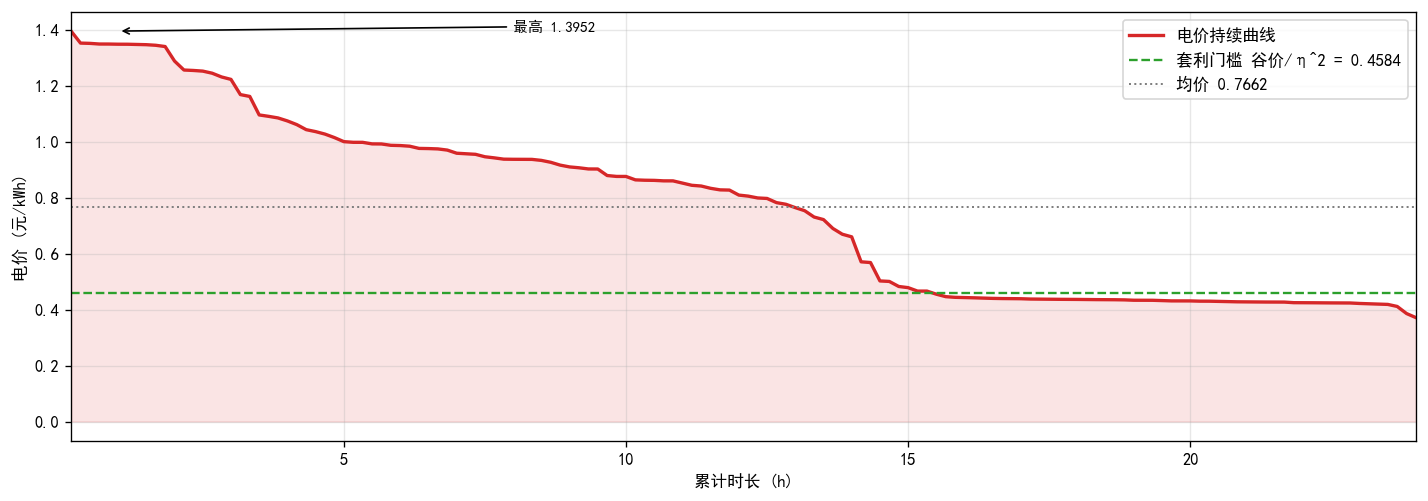
\includegraphics[width=\textwidth]{套利门槛.png}
    \subcaption{电价持续时长曲线}
\end{minipage}
\caption{变量相关性与电价持续时长}
\end{figure}

热力图显示：光伏功率与净负荷（负载 $-$ 光伏）呈强负相关，故将二者合并为净负荷可降低后续建模复杂度；电价与小区负载正相关，即用电高峰往往伴随高电价，进一步说明引入储能的必要性。电价持续时长曲线给出了峰、平、谷三段的累计小时数，可用于判断“套利门槛”（充放电循环的价差需覆盖 $\eta$ 造成的能量损失）是否被满足。

\subsection{预报精度指标（MAE / RMSE / 偏差）的定义与口径}
本文多处用 MAE 比较预报方法，故先给出统一定义与三条口径，后续引用不再重复。

\noindent\textbf{(1) 误差与指标.}设第 $d$ 天第 $t$ 个时段（$t=1,\dots,144$）的实际值与预报值分别为 $x_{d,t}$ 与 $\hat x_{d,t}$（均为功率，单位 kW），误差记为 $\varepsilon_{d,t}$（注意：全文的 $e_t$ 专指\textbf{紧急购电功率}，两者不可混用）：
\begin{equation}
    \varepsilon_{d,t}=x_{d,t}-\hat x_{d,t},
\end{equation}
四个指标出自同一个误差样本：
\begin{align}
    \mathrm{MAE}&=\frac{1}{N}\sum_{d=1}^{D}\sum_{t=1}^{T}\bigl|\varepsilon_{d,t}\bigr|, &
    \mathrm{RMSE}&=\sqrt{\frac{1}{N}\sum_{d=1}^{D}\sum_{t=1}^{T}\varepsilon_{d,t}^{2}},\\
    \mathrm{bias}&=\frac{1}{N}\sum_{d=1}^{D}\sum_{t=1}^{T}\varepsilon_{d,t}, &
    \sigma&=\sqrt{\frac{1}{N}\sum_{d=1}^{D}\sum_{t=1}^{T}\bigl(\varepsilon_{d,t}-\mathrm{bias}\bigr)^{2}},
\end{align}
其中 $N=DT$ 为参与统计的「天 $\times$ 时段」对数。按此定义，$\mathrm{bias}>0$ 表示\textbf{低估}（实际大于预报）。7.3 与 8.3 节报童裕量所用的历史误差 $\varepsilon_{j,t}$（$j<d$ 为历史日）与此同记号、同含义。

\noindent\textbf{(2) 平均方式.}式 (13) 采用“先展平再平均”。由于每天恰有 $T=144$ 个时段，它与“先按日求 MAE、再对日平均”在数值上\textbf{完全相等}（实测两者均为 $132.732234$），故两种读法不会产生差异。

\noindent\textbf{(3) 统计范围.}第 $h\in\{0,6,12,18\}$ 个决策时刻发布的预报，只统计\textbf{该时刻尚未发生}的时段：
\begin{equation}
    \mathrm{MAE}_h=\frac{1}{N_h}\sum_{d=1}^{D}\ \sum_{t=6h+1}^{144}\bigl|x_{d,t}-\hat x^{(h)}_{d,t}\bigr|,
    \qquad N_h=D\,(144-6h).
\end{equation}
原因是构造预报时会把已发生时段的实际值直接填入（该段误差恒为 $0$），若不分段统计，指标会被这批“必然为零”的点稀释：以 6:00 为例，算满 144 槽得 $118.57$ kW，只算其后的 108 槽才是 $158.09$ kW。

\noindent\textbf{(4) 统计窗口.}主口径取与结果一致的 \textbf{2025-02-01 起 334 天}，此时 $N=334\times144=48\,096$；若取全 365 天（含前 31 天预热期，其历史样本不足），同一指标的数值会系统性偏低 $4\sim6$ kW。因此两套数字不得混用，凡引用一律注明窗口。

\begin{table}[htbp]
\centering
\caption{\textbf{预报精度指标的口径与实测值（问题三光伏预报，0:00 发布版，$m=0.4$）}}
\label{tab:mae_def}
\small
\begin{tabular}{|l|r|r|r|r|r|}
\hline
统计范围 & 参与时段数 & 样本数 $N$ & MAE (kW) & 平均偏差 (kW) & 标准差 (kW) \\
\hline
0:00 发布（全天 144 槽） & 144 & 48\,096 & 132.73 & $+10.97$ & 261.04 \\
\hline
6:00 发布（其后的 108 槽） & 108 & 36\,072 & 158.09 & $-4.89$ & --- \\
\hline
12:00 发布（其后的 72 槽） & 72 & 24\,048 & 108.97 & $+10.22$ & --- \\
\hline
18:00 发布（其后的 36 槽） & 36 & 12\,024 & 7.80 & $+7.76$ & --- \\
\hline
\end{tabular}
\end{table}

\noindent\textbf{(5) 误差分布特征：为什么 MAE 不能直接当决策目标.}以 0:00 发布版为例，$\mathrm{MAE}/\sigma=0.508$，远低于正态分布的理论值 $\sqrt{2/\pi}=0.798$，峰度为 10.1（正态为 3）；$41.5\%$ 的样本误差恰为 $0$（夜间光伏恒为 0），白天（$6{:}00\sim18{:}00$）MAE 为 260.69 kW，夜间仅 4.78 kW；$|e|$ 的中位数、90\% 分位与 99\% 分位分别为 14.9、438.8、1001.5 kW，最大 1994.2 kW。可见误差呈\textbf{尖峰厚尾}分布：MAE 把大量零误差点与白天的大误差一并平均，且对正负一视同仁；而费用函数是\textbf{不对称}的 —— 低估光伏只是多买（代价约 $\pi_t$），高估光伏会留下缺口、须按 $5\pi_t$ 紧急补足。故本文只用 MAE 筛选候选参数，最终定参一律以全年购电费用为准（见 8.2.3 节与 10.4 节）。

\section{问题一模型的建立与求解}
\subsection{模型建立}
在电价、负载、光伏预测均已知的条件下，决策变量为各时段购电功率 $b_t$、充放电功率 $c_t,d_t$、弃光功率 $s_t$ 与储能电量 $E_t$，目标是全天购电费用最小。

\subsection{约束条件}
\begin{enumerate}
    \item \textbf{功率平衡约束：}题目要求微网提供的电能不低于小区负载。引入弃光变量 $s_t$ 后（光伏过剩且储能充满时必须有消纳出口，否则可行域为空），平衡式可写为等式：
    \begin{equation}
        b_t+\hat G_t+d_t-c_t-s_t = L_t, \qquad t=1,\dots,T.
    \end{equation}
    \item \textbf{储能状态转移方程：}
    \begin{equation}
        E_t=E_{t-1}+\left(\eta c_t-\frac{d_t}{\eta}\right)\Delta t,\qquad t=1,\dots,T,\quad E_0=6000\ \text{kWh}.
    \end{equation}
    \item \textbf{SOC 安全区间：}$E_{\min}\le E_t\le E_{\max}$。
    \item \textbf{始末电量守恒：}$E_T=E_0=6000$ kWh。
    \item \textbf{充放电功率上限与互斥：}
    \begin{equation}
        0\le c_t\le u_t P_{\max},\qquad 0\le d_t\le (1-u_t)P_{\max},\qquad u_t\in\{0,1\}.
    \end{equation}
    \item \textbf{非负性：}$b_t\ge0,\ s_t\ge0$。
\end{enumerate}

\subsection{目标函数}
\begin{equation}
    \min\ Z=\sum_{t=1}^{T}\pi_t\, b_t\,\Delta t
    \label{eq:q1_obj}
\end{equation}
其中 $T=144$、$\Delta t=1/6$ h。需要强调：若要报出“全天购电量（kWh）”，必须使用 $\sum_t b_t\Delta t$（$b_t$ 是功率），不能直接把 144 个功率值相加；本文的程序中该量由 \texttt{q\_buy\ =\ p\_buy*DT\_H} 统一换算，避免量纲混淆。

\subsection{模型求解与结果}
用 Python 的 PuLP 建模、CBC 求解器求解，得到全局最优解。全天结果如下：

\begin{itemize}
    \item 全天总购电量 \textbf{59\,482.6990 kWh}，全天总购电费 \textbf{35\,126.9486 元}；
    \item 平均购电单价 $35\,126.9486/59\,482.6990=0.5906$ 元/kWh，比电价均值 0.7662 元/kWh 低 22.9\%；
    \item 全天负载 111\,024.8 kWh、光伏（附件 1 预测）55\,482.8 kWh、净负荷 55\,542.0 kWh；
    \item 储能全天充电 20\,740.67 kWh、放电 16\,799.94 kWh，\textbf{净充电} 3\,940.73 kWh。购电量 59\,482.7 kWh 高于净负荷 55\,542.0 kWh，差额恰为 3\,940.7 kWh，即“谷段多买、存入储能”，这直接验证了套利机制的存在。
\end{itemize}

\begin{table}[htbp]
\centering
\caption{\textbf{微网在指定时间段的购电量及全天购电量、购电费（问题一）}}
\label{tab:q1_buy}
\small
\begin{tabular}{|c|c|c|c|c|c|c|}
\hline
时间段 & 购电量(kWh) & 时间段 & 购电量(kWh) & 时间段 & 购电量(kWh) \\
\hline
10:00-10:10 & 0.0000 & 12:00-12:10 & 480.4125 & 14:00-14:10 & 0.0000 \\
\hline
16:00-16:10 & 445.4316 & 18:00-18:10 & 531.8940 & 20:00-20:10 & 0.0000 \\
\hline
\multicolumn{2}{|c|}{全天购电量 59\,482.6990 kWh} & \multicolumn{2}{c|}{全天购电费 35\,126.9486 元} & \multicolumn{2}{c|}{平均单价 0.5906 元/kWh} \\
\hline
\end{tabular}
\end{table}

\begin{table}[htbp]
\centering
\caption{\textbf{储能设备在指定时间段的充放电量及 0:00 与 24:00 的储电量（问题一）}}
\label{tab:q1_soc}
\small
\begin{tabular}{|c|c|c|c|c|c|}
\hline
时间段 & 充电量(kWh) & 放电量(kWh) & 时间段 & 充电量(kWh) & 放电量(kWh) \\
\hline
0:00-4:00   & 4500.0000 & 0.0000    & 4:00-8:00   & 833.3333  & 6365.8412 \\
\hline
8:00-12:00  & 4787.9643 & 1702.9970 & 12:00-16:00 & 5286.0352 & 91.1014 \\
\hline
16:00-20:00 & 0.0000    & 5780.1319 & 20:00-24:00 & 5333.3333 & 2859.8681 \\
\hline
\multicolumn{2}{|c|}{0:00 储电量} & 6000.0000 kWh & \multicolumn{2}{c|}{24:00 储电量} & 6000.0000 kWh \\
\hline
\end{tabular}
\end{table}

\subsection{命题：$\eta<1$ 时充放电互斥约束可松弛}
\textbf{命题.} 若 $\eta<1$，则约束 (5) 中的 $u_t$ 可以松弛为 $u_t\equiv1$（即删除该约束）而不改变最优值。

\noindent\textbf{证明.} 设某最优解在时段 $t$ 同时有 $c_t>0,\ d_t>0$，令 $m=\min(\eta c_t,\ d_t/\eta)>0$。把 $c_t$ 减少 $m/\eta$、$d_t$ 减少 $m\eta$，则状态转移式 (2) 中 $\eta c_t-d_t/\eta$ 的变化为 $-m+m=0$，即 $E_t$ 不变；而功率平衡式 (1) 中 $b_t$ 需增加 $(m/\eta-m\eta)=(1-\eta^2)m/\eta>0$，目标函数 (1) 也随之增大，与原解最优矛盾（若原解中 $b_t$ 已为 0，则该时段不平衡量转由减少弃光承担，目标函数不增大而 $s_t$ 减小，属于等价最优解，可通过取 $c_t=\min(c_t,d_t/\eta\cdot\eta)$ 消除）。故最优解满足 $c_t d_t=0$。$\square$

\noindent\textbf{数值验证.} 分别用 MILP（含 144 个 0-1 变量）与 LP（删除 $u_t$）求解问题一：两者目标值均为 35\,126.9486 元（差 0.0），全天购电量均为 59\,482.6990 kWh，逐时段 $b_t,c_t,d_t$ 的最大差异为 $0$，且 LP 解中同时充放电的时段数为 $0$。这验证了命题，也说明问题二至问题四使用纯 LP 是合理的。

\subsection{结果分析}
优化结果呈现清晰的“谷充峰放”结构：凌晨 $0{:}00\sim4{:}00$ 为电价谷段，储能以接近额定功率充电 4500 kWh；$4{:}00\sim8{:}00$ 与 $16{:}00\sim20{:}00$ 为电价峰段，储能大量放电（6365.8 与 5780.1 kWh）以替代高价购电；$8{:}00\sim12{:}00$ 与 $12{:}00\sim16{:}00$ 光伏充足，储能吸纳盈余并部分放电。$10{:}00\sim10{:}10$、$14{:}00\sim14{:}10$、$20{:}00\sim20{:}10$ 三个抽样时段的购电量为 0，说明这些时段由光伏与储能完全覆盖。

\noindent\textbf{对照实验.}为说明“优化”相对于“经验规则”的价值，本文设置三组对照：无储能（按净负荷直接购电）、固定时段“谷充峰放”规则（谷段满充、峰段满放，不看净负荷）、以及本文优化模型。结果见表 \ref{tab:q1_ab} 与图 \ref{fig:q1_ab}。

\begin{table}[htbp]
\centering
\caption{\textbf{问题一三种策略的对照实验结果}}
\label{tab:q1_ab}
\small
\begin{tabular}{|l|r|r|r|r|r|}
\hline
策略 & 购电费(元) & 购电量(kWh) & 光伏消纳率 & 峰段占比 & 弃光(kWh) \\
\hline
无储能 & 48\,052.05 & 61\,789.94 & 88.7\% & 30.1\% & 6\,247.96 \\
\hline
规则谷充峰放 & 52\,695.81 & 76\,166.79 & 76.4\% & 21.6\% & 13\,106.48 \\
\hline
优化模型（本文） & \textbf{35\,126.95} & 59\,482.70 & \textbf{100.0\%} & \textbf{13.1\%} & \textbf{0.00} \\
\hline
\end{tabular}
\end{table}

值得强调的是：朴素的“谷充峰放”规则（52\,695.81 元）反而比根本不装储能（48\,052.05 元）更贵。原因是该规则不看净负荷，在凌晨盲目满充，导致白天光伏无处吸纳而弃光 13\,106 kWh，同时又在峰段被迫与光伏重复供给。而本文优化模型同时做到“光伏 100\% 消纳、零弃光、峰段购电占比仅 13.1\%”，比无储能省 12\,925.10 元（26.90\%），比规则型省 17\,568.86 元（33.34\%）。

\begin{figure}[htbp]
\centering
\begin{minipage}[c]{0.62\textwidth}
    \centering
    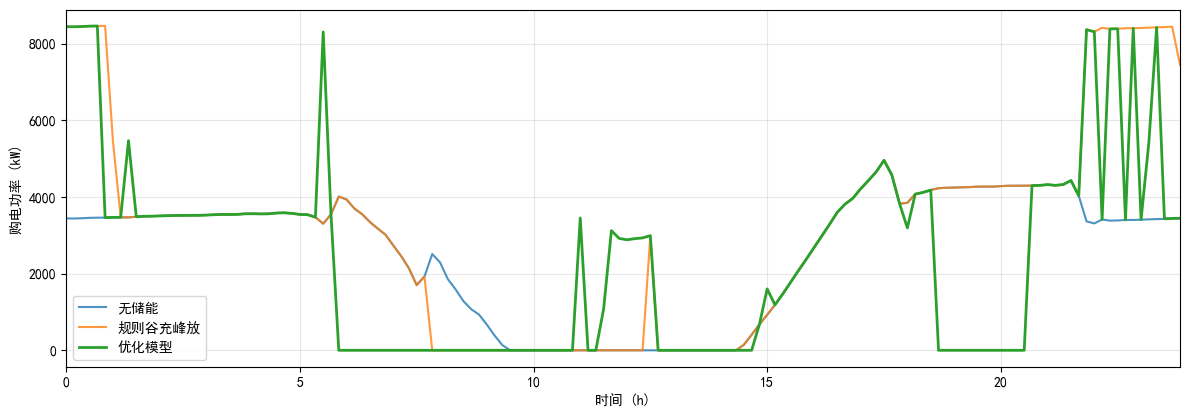
\includegraphics[width=\textwidth]{问题一_购电对比.png}
    \subcaption{三种策略的购电功率曲线}
\end{minipage}\hfill
\begin{minipage}[c]{0.35\textwidth}
    \centering
    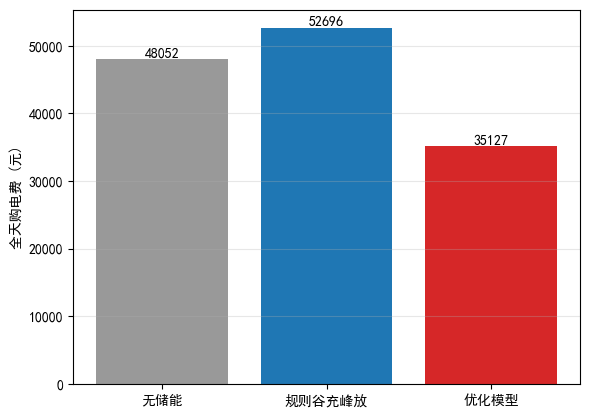
\includegraphics[width=\textwidth]{问题一_费用对比.png}
    \subcaption{全天购电费对比}
\end{minipage}
\caption{问题一的对照实验：无储能 / 规则谷充峰放 / 优化模型}
\label{fig:q1_ab}
\end{figure}

\begin{figure}[htbp]
\centering
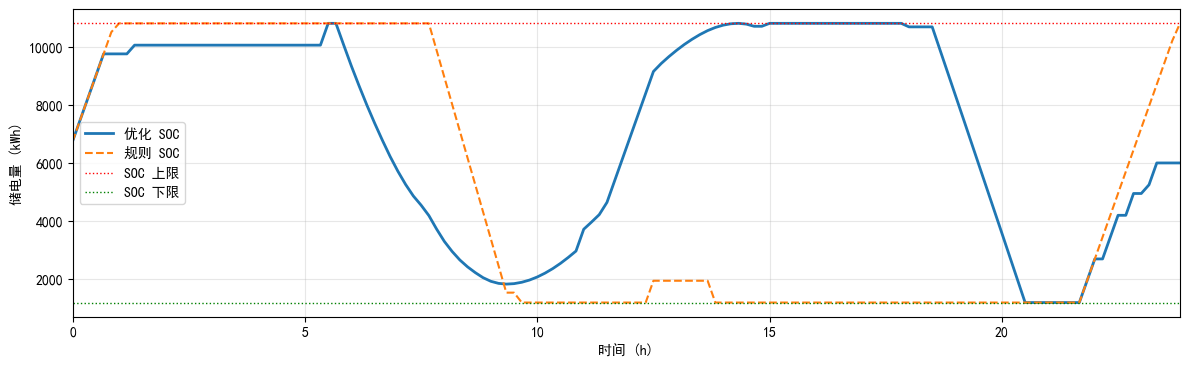
\includegraphics[width=0.76\textwidth]{问题一_SOC对比.png}
\caption{三种策略的储能 SOC 轨迹：优化模型在谷段充满、峰段放空，且在 24:00 严格回到 6000 kWh}
\label{fig:q1_soc}
\end{figure}

\section{问题二模型的建立与求解}
\subsection{模型建立}
问题二中电价固定（附件 1），但负载与光伏逐日逐时段波动且事先未知。计划购电量 $b_t$ 在 0:00 锁定后不可更改；实际执行时若出现缺口，先由储能放电、再由紧急购电（$5\pi_t$）补足。因此模型分两阶段：\textbf{第一阶段}用日前预测加报童裕量制定计划，\textbf{第二阶段}以“逐槽被动平衡”模拟储能实时动作。

\subsection{不确定性因素的定义与预测}
\subsubsection{小区负载预测：为什么用“上周同一天”}
\begin{figure}[htbp]
\centering
\begin{minipage}[c]{0.48\textwidth}
    \centering
    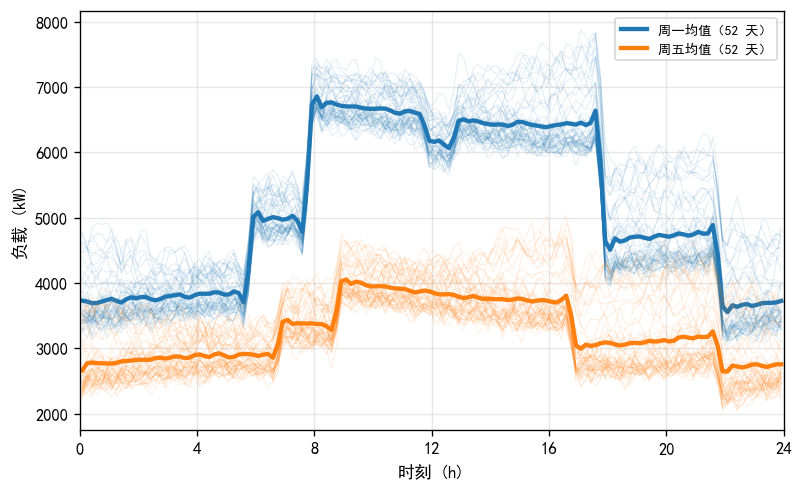
\includegraphics[width=\textwidth]{负载同星期叠加.png}
    \subcaption{同一星期几的负载曲线叠加}
\end{minipage}\hfill
\begin{minipage}[c]{0.48\textwidth}
    \centering
    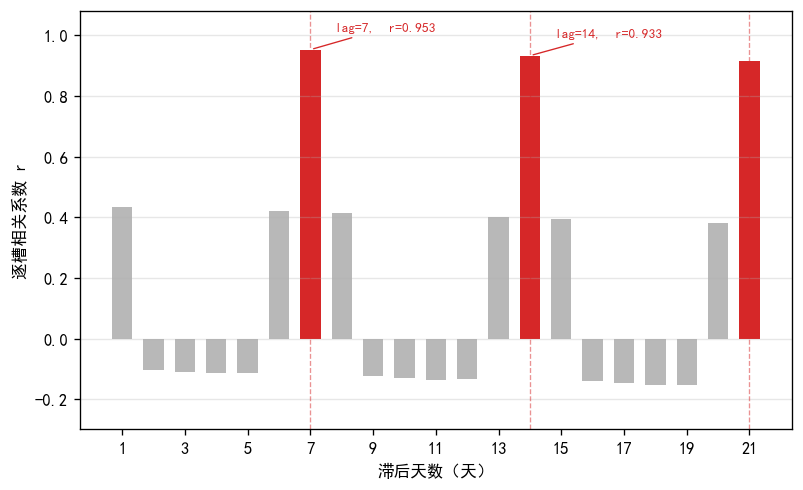
\includegraphics[width=\textwidth]{负载自相关系数.png}
    \subcaption{负载的自相关系数（滞后 7 天出现孤立峰值）}
\end{minipage}
\caption{小区负载周期性验证}
\end{figure}

把全年同一星期几的负载曲线叠加后可见，同一天内历史各周的波动很小；日总量自相关在滞后 7 天处出现孤立峰值 $r=0.988$，而滞后 1 天仅 $0.374$、滞后 3 天为 $-0.258$，呈明显的\textbf{周季节性}。故采用“上周同一天”作为日前预测：
\begin{equation}
\hat L_{d,t}=
\begin{cases}
L^{\mathrm{real}}_{d-7,t}, & d\ge 7,\\
L^{\mathrm{att1}}_{t}, & d<7
\end{cases}
\end{equation}
（输出窗口自 2025-02-01 起，故实际全部使用历史周数据。）

\subsubsection{光伏发电预测：为什么用“前 3 天滑动平均”}
光伏不具备周周期：其日总量自相关在滞后 1 天达 $0.964$，滞后 7 天仅 $0.929$，没有孤立峰值，故不能照搬“上周同一天”。本文对滑窗 $k_w=1,\dots,10$ 做了双重检验（\texttt{q2\_光伏预报方法.txt}，图 \ref{fig:pvwin}；MAE 口径见 5.3 节）：

\begin{center}
\small
\begin{tabular}{cccccccc}
\hline
滑窗 $k_w$ & 1 & 2 & 3 & 4 & 5 & 7 & 10 \\
\hline
MAE (kW) & 185.3 & 162.1 & 154.5 & 151.9 & 151.5 & 153.4 & 159.8 \\
全年费用 (万元) & 1404.6 & 1397.5 & \textbf{1394.9} & 1393.9 & 1396.8 & 1397.4 & 1400.5 \\
\hline
\end{tabular}
\end{center}

可以看出：单日持续性预报（$k_w=1$）的 MAE 比 $k_w=3$ 差 20.0\%，说明单日跟不上天气突变；但窗口拉到 7$\sim$10 天又过度平滑而变差。MAE 最小点在 $k_w=5$、全年费用最小点在 $k_w=4$，两者相差仅 0.07\%（9\,851.8 元），属于噪声水平。因此严谨的表述是：\textbf{$k_w=3\sim7$ 构成平坦平台}，平台内任意取值都可接受，本文取 $k_w=3$ 以兼顾简洁与稳定（作为对照，若完全弃用近期历史、改用附件 1 的“气候态基准日”，费用将升至 14\,839\,836.8 元，高 6.39\%）。

\begin{equation}
\hat G_{d,t}=\frac{1}{\min(d,k_w)}\sum_{j=1}^{\min(d,k_w)}G^{\mathrm{real}}_{d-j,t},\qquad k_w=3.
\end{equation}
\begin{figure}[htbp]
\centering
\begin{minipage}[c]{0.48\textwidth}
    \centering
    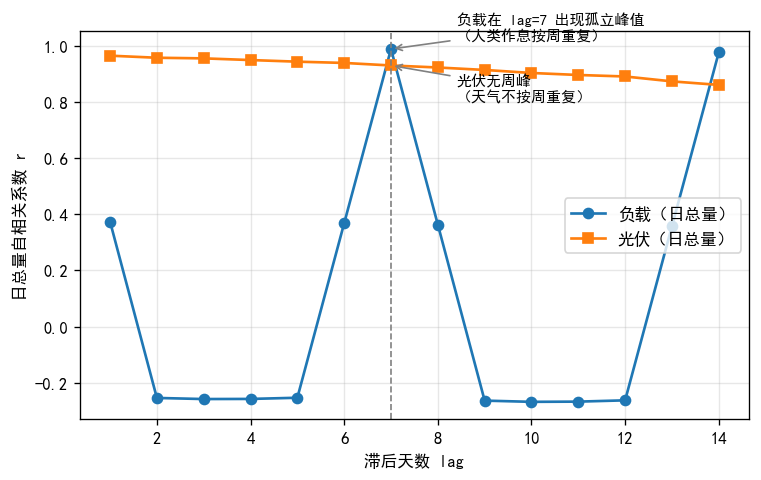
\includegraphics[width=\textwidth]{光伏滞后自相关.png}
    \subcaption{负载与光伏的滞后自相关}
\end{minipage}\hfill
\begin{minipage}[c]{0.48\textwidth}
    \centering
    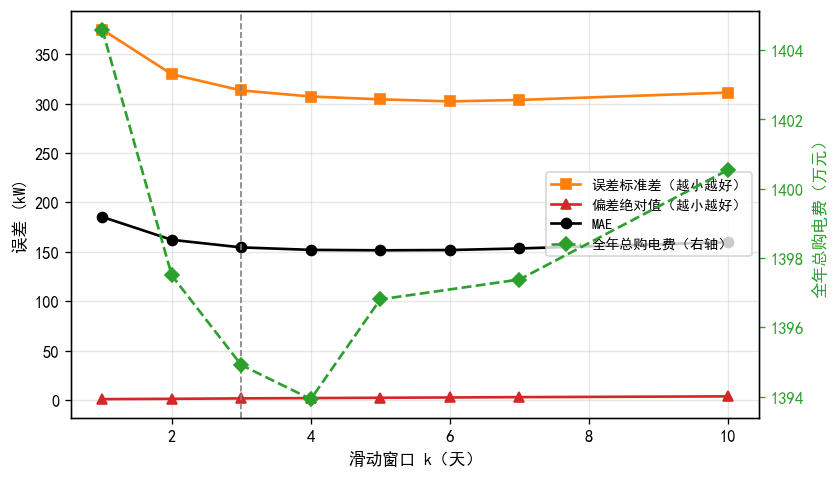
\includegraphics[width=\textwidth]{光伏窗口扫描.png}
    \subcaption{滑窗扫描：MAE 与全年费用}
\end{minipage}
\caption{光伏预报窗口的定参依据}
\label{fig:pvwin}
\end{figure}

\begin{figure}[htbp]
\centering
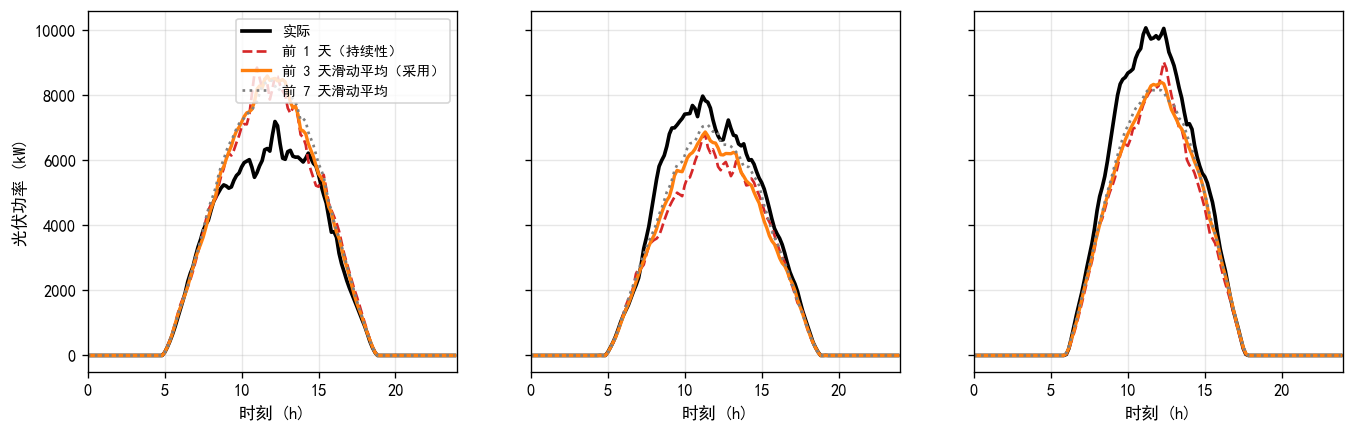
\includegraphics[width=0.8\textwidth]{光伏典型日预报对比.png}
\caption{典型日的预报对比：单日持续性预报跟不上天气突变，7 天平均又过度平滑，3 天滑窗处于两者之间}
\label{fig:pvday}
\end{figure}

\subsection{报童模型与安全裕量}
设第 $d$ 天第 $t$ 时段的预测净负荷为
\begin{equation}
    Net^{\mathrm{pred}}_{d,t}=\hat L_{d,t}-\hat G_{d,t}.
\end{equation}
若按预测值购电，则实际净负荷高于预测时产生紧急购电。以“多买 1 kWh”成本 $c_o=\pi_t$、“少买 1 kWh”的净损失 $c_u=5\pi_t-\pi_t=4\pi_t$，由报童模型临界分位数公式
\begin{equation}
    \alpha^{*}=\frac{c_u}{c_u+c_o}=\frac{4\pi_t}{4\pi_t+\pi_t}=0.80,
\end{equation}
即计划购电量应覆盖历史预测误差的 80\% 分位数。历史净负荷预测误差样本为
\begin{equation}
    \varepsilon_{j,t}=(L^{\mathrm{real}}_{j,t}-G^{\mathrm{real}}_{j,t})-(\hat L_{j,t}-\hat G_{j,t}),
\end{equation}
取过去 $W$ 天（严格只用 $j<d$，避免使用未来信息）的 $\alpha^{*}$ 分位数作为裕量：
\begin{equation}
    X_{d,t}=\mathrm{Quantile}_{\alpha^{*}}\bigl(\{\varepsilon_{j,t}\mid \max(0,d-W)\le j<d\}\bigr),
    \qquad
    \tilde L_{d,t}=\hat L_{d,t}+X_{d,t}.
\end{equation}

\textbf{参数定标.} 由 4.3 节可知费用对分位数并不敏感（$0.80$ 与最优的 $0.76$ 相差 0.12\%），窗口 30 天与 60 天相差 0.22\%。本文最终采用 $\alpha^{*}=0.76$、$W=30$，日均裕量 251 kW、最大 3\,672 kW；若完全不设裕量（$X\equiv0$），全年费用将升至 15\,228\,314.3 元，比本方案高 127.9 万元（8.40\%），说明报童裕量的价值远大于其参数误差带来的波动。

\subsection{约束条件}
\begin{enumerate}
    \item \textbf{日前功率平衡（第一阶段）：}
    \begin{equation}
        b_t+\hat G_{d,t}+d_t-c_t-s_t\ \ge\ \tilde L_{d,t},\qquad \forall t=1,\dots,144 .
    \end{equation}
    此处采用“$\ge$”而非“$=$”：由于购电量 $b_t$ 的系数为正，最优解不会多余购电，故不等式在最优处取等号；保留不等式形式可避免浮点误差导致不可行。
    \item \textbf{储能状态转移与容量约束：}$E_t=E_{t-1}+(\eta c_t-d_t/\eta)\Delta t$，$E_{\min}\le E_t\le E_{\max}$，$E_0$ 取当天初值。
    \item \textbf{功率与非负约束：}$0\le c_t,d_t\le P_{\max}$，$b_t,s_t\ge0$。
\end{enumerate}

\subsection{模型求解}
\noindent\textbf{(a) 第一阶段：日前线性规划.}
\begin{equation}
    \min\ \sum_{t=1}^{144}\pi_t\,b_t\,\Delta t
\end{equation}

\noindent\textbf{(b) 第二阶段：逐槽被动平衡（实际执行）.}购电量锁定为 $b_t$ 后，储能只能被动平衡，实时净偏差为
\begin{equation}
    \Delta P_t=L^{\mathrm{real}}_t-G^{\mathrm{real}}_t-b_t .
\end{equation}
\begin{itemize}
    \item 若 $\Delta P_t>0$（缺电）：先放电补缺，放电受功率与剩余电量双约束
    \begin{equation}
        d_t=\min\left(\Delta P_t,\ P_{\max},\ \frac{(E_{t-1}-E_{\min})\eta}{\Delta t}\right),\qquad
        e_t=\Delta P_t-d_t ;
    \end{equation}
    \item 若 $\Delta P_t<0$（盈余）：先充电吸纳，充电受功率与剩余空间双约束
    \begin{equation}
        c_t=\min\left(-\Delta P_t,\ P_{\max},\ \frac{E_{\max}-E_{t-1}}{\eta\Delta t}\right),\qquad
        s_t=-\Delta P_t-c_t ;
    \end{equation}
    \item 状态更新 $E_t=E_{t-1}+(\eta c_t-d_t/\eta)\Delta t$，递推至 $t=144$。

    该规则不含前瞻，因此“全天仿真”与“分段仿真拼接”完全一致，逐日滚动时只需把当天 24:00 的 $E$ 作为次日初值。
\end{itemize}

全天费用由三部分构成：
\begin{equation}
    C=\underbrace{\sum_t \pi_t b_t\Delta t}_{\text{计划购电费}}+\underbrace{\sum_t 5\pi_t e_t\Delta t}_{\text{紧急购电费}} .
\end{equation}

\subsection{求解结果}
逐日滚动求解 365 天（前 31 天为预热期），统计窗口内 334 天结果如下：

\begin{center}
\begin{tabular}{lrlr}
\hline
指标 & 数值 & 指标 & 数值 \\
\hline
计划购电量 & 21\,442\,248.8 kWh & 计划购电费 & 13\,155\,069.0 元 \\
紧急购电量 & 141\,988.6 kWh（0.66\%） & 紧急购电费 & 794\,039.5 元 \\
\textbf{总购电费} & \textbf{13\,949\,108.5 元} & 出现紧急购电天数 & 141 / 334 天 \\
\hline
\end{tabular}
\end{center}

若不计储能、直接按净负荷购电，全年需 16\,407\,319.6 元，故储能与裕量机制合计节省 245.8 万元（15.0\%）。需要指出，紧急购电仅占总购电量的 0.66\%，却贡献了 5.7\% 的费用，说明惩罚电价对费用的放大作用——这正是设置安全裕量的意义。

\begin{table}[htbp]
\centering
\caption{\textbf{微网在指定时间段的购电量及全天购电量、购电费（问题二，单位：kWh / 元）}}
\label{tab:q2_buy}
\adjustbox{max width=\textwidth}{%
\begin{tabular}{|c|c|c|c|c|}
\hline
时间段 & 2025.3.20 & 2025.6.21 & 2025.9.23 & 2025.12.21 \\
\hline
10:00-10:10 & 0.00 & 0.00 & 0.00 & 0.00 \\
\hline
12:00-12:10 & 517.65 & 0.00 & 492.71 & 949.98 \\
\hline
14:00-14:10 & 0.00 & 0.00 & 0.00 & 0.00 \\
\hline
16:00-16:10 & 482.80 & 251.37 & 572.00 & 832.47 \\
\hline
18:00-18:10 & 713.46 & 0.00 & 778.58 & 739.25 \\
\hline
20:00-20:10 & 0.00 & 0.00 & 0.00 & 0.00 \\
\hline
全天计划购电量 & 66\,488.47 & 35\,893.66 & 69\,314.94 & 98\,714.56 \\
\hline
全天计划购电费 & 40\,578.62 & 21\,555.82 & 43\,159.88 & 63\,810.09 \\
\hline
\end{tabular}
}
\end{table}

\begin{table}[htbp]
\centering
\caption{\textbf{储能设备在指定时间段的充放电量及 0:00 与 24:00 的储电量（问题二，单位：kWh）}}
\label{tab:q2_soc}
\adjustbox{max width=\textwidth}{%
\begin{tabular}{|c|c|c|c|c|c|c|c|c|}
\hline
\multirow{2}{*}{时间段} & \multicolumn{2}{c|}{2025.3.20} & \multicolumn{2}{c|}{2025.6.21} & \multicolumn{2}{c|}{2025.9.23} & \multicolumn{2}{c|}{2025.12.21} \\
\cline{2-9}
 & 充电量 & 放电量 & 充电量 & 放电量 & 充电量 & 放电量 & 充电量 & 放电量 \\
\hline
0:00-4:00   & 8\,107.62 & 148.27   & 950.78   & 40.96    & 9\,084.30 & 17.46    & 8\,785.71 & 82.84 \\
\hline
4:00-8:00   & 1\,927.53 & 5\,496.18 & 696.15   & 1\,753.53 & 1\,607.22 & 6\,086.27 & 2\,084.29 & 1\,446.15 \\
\hline
8:00-12:00  & 5\,939.23 & 2\,777.38 & 8\,929.75 & 0.00     & 5\,213.17 & 1\,896.62 & 5\,689.53 & 6\,847.20 \\
\hline
12:00-16:00 & 4\,402.48 & 503.91   & 0.00     & 0.00     & 4\,693.24 & 583.67   & 6\,512.22 & 2\,220.11 \\
\hline
16:00-20:00 & 268.61    & 5\,654.08 & 201.45   & 5\,184.72 & 271.23    & 5\,678.20 & 3.13     & 5\,633.87 \\
\hline
20:00-24:00 & 603.28    & 2\,979.55 & 1\,479.26 & 2\,485.90 & 732.29    & 2\,894.74 & 597.69   & 2\,859.78 \\
\hline
0:00 储电量  & \multicolumn{2}{c|}{2\,101.44} & \multicolumn{2}{c|}{3\,274.87} & \multicolumn{2}{c|}{1\,394.58} & \multicolumn{2}{c|}{1\,809.09} \\
\hline
24:00 储电量 & \multicolumn{2}{c|}{1\,714.91} & \multicolumn{2}{c|}{3\,789.73} & \multicolumn{2}{c|}{1\,772.60} & \multicolumn{2}{c|}{1\,903.36} \\
\hline
\end{tabular}
}
\end{table}

\begin{table}[htbp]
\centering
\caption{\textbf{微网在指定日期的紧急购电量（问题二，单位：kWh）}}
\label{tab:q2_emg}
\begin{tabular}{|c|c|c|c|c|}
\hline
日期 & 时间段 & 紧急购电量 & 当日合计 & 说明 \\
\hline
2025.3.20 & --- & --- & 0.00 & 无紧急购电 \\
\hline
2025.6.21 & --- & --- & 0.00 & 无紧急购电 \\
\hline
\multirow{4}{*}{2025.9.23} & 20:20-20:40 & 145.36 & \multirow{4}{*}{209.62} & \\
 & 20:50-21:10 & 47.01 & & 晚高峰光伏已无出力 \\
 & 21:20-21:30 & 17.25 & & 且储能已放至下限 \\
\hline
2025.12.21 & --- & --- & 0.00 & 无紧急购电 \\
\hline
\end{tabular}
\end{table}

\subsection{结果分析}
四个指定日期中仅 2025-09-23 出现紧急购电（209.62 kWh），且全部落在 $20{:}20\sim21{:}30$：此时光伏已无出力、储能电量已接近下限，而实际负载高于按“上周同一天”得到的预测值。其余三个日期预测误差较小，储能放电压住了全部缺口。储能方面，春季与冬季的充电集中在凌晨谷段（8\,107.62 与 8\,785.71 kWh），放电集中在 $4{:}00\sim8{:}00$、$16{:}00\sim20{:}00$ 两个峰段；夏季（6.21）光伏充裕，$8{:}00\sim16{:}00$ 以充电为主、放电为 0，呈现典型的“消纳为主、套利为辅”特征。

\section{问题三模型的建立与求解}
\subsection{模型建立}
问题三与问题二的差别有两处：（1）光伏预报在 0:00、6:00、12:00、18:00 四次更新，决策可随之滚动调整；（2）对计划的任何偏离都要付惩罚费用——下调违约按 $0.5\pi_t$、上调超出按 $1.5\pi_t$。
于是同一时段的购电费用（相对计划量 $b^p_t$ 与调整量 $b^a_t$）为
\begin{equation}
    C_t=\pi_t\min(b^p_t,b^a_t)+0.5\pi_t\,(b^p_t-b^a_t)^{+}+1.5\pi_t\,(b^a_t-b^p_t)^{+},
    \label{eq:q3_cost}
\end{equation}
它是关于 $b^a_t$ 的凸分段线性函数，可用偏差变量 $\delta^{\pm}$ 线性化：
\begin{equation}
    C_t=\pi_t b^p_t+1.5\pi_t\delta^{+}_t-0.5\pi_t\delta^{-}_t,\qquad
    b^a_t=b^p_t+\delta^{+}_t-\delta^{-}_t,\qquad \delta^{\pm}_t\ge0 .
\end{equation}

\noindent\textbf{量纲说明.}式中的 $b^p_t,b^a_t,\delta^{\pm}_t$ 沿用符号表的功率记号（kW），
故 $C_t$ 是\textbf{费用率}（元/h），该时段的实际电费为 $C_t\,\Delta t$；
等价地，若把 $b^p_t,b^a_t$ 换成该时段的\textbf{电量}（kWh，即功率 $\times\Delta t$），
则上式直接给出电费（元）。交付文件 \texttt{result3.xlsx} 采用后一种口径，
本文正文表格均报时段的电量与电费。

\subsection{不确定性因素与预报构造}
负载预测仍用“上周同一天”，并加入\textbf{当日自适应修正}：用当天已发生时段的实际值与预报值之比（限幅 $\pm20\%$）缩放剩余时段的预报。这是真实可得的增量信息（无需额外预报），实测使剩余时段 MAE 由 198.4 kW 降至 172.9 kW（降 12.9\%）。
\subsubsection{光伏预报的混合：为什么取 $m=0.4$}
光伏有两个信息来源：附件 3 的短期预报（每天 4 次发布，跟随天气形势，但带随机误差）与历史外推（前 3 天滑动平均，只反映近期气候态）。二者单独使用都不理想，本文先量化其误差结构，再用\textbf{方差最小化}定出权重，而不是凭试算挑。

\noindent\textbf{(1) 两种基础预报的误差结构.}为便于比较，统一按 0:00 发布的那一版预报评价（覆盖全天 144 个时段），指标定义在结果窗口 \textbf{2025-02-01 起 334 天}上，口径见 5.3 节：

\begin{center}
\small
\begin{tabular}{lrrrr}
\hline
预报来源 & MAE (kW) & RMSE (kW) & 平均偏差 (kW) & 误差标准差 (kW) \\
\hline
附件 3 单用（$m=1$） & 197.5 & 383.0 & $+29.7$ & 373.6 \\
前 3 天滑动平均（$m=0$） & 154.5 & 313.5 & $-1.5$ & 305.2 \\
\hline
\end{tabular}
\end{center}

可见：附件 3 虽然“知道”当天的天气形势，但它的\textbf{随机误差更大}（标准差 373.6 kW，比历史外推高 22.4\%），且带明显负偏差 $+29.7$ kW（偏差取自“实际 $-$ 预报”，正值表示\textbf{系统性低估}光伏）；纯历史外推几乎无偏（$-1.5$ kW）但同样不够准。关键在于两者的误差近似独立：$\rho(e_{\mathrm{att3}},e_{\mathrm{hist}})=+0.165$，只弱相关，因此\textbf{加权平均可以让随机误差相互抵消}，这正是混合有效的前提。

\noindent\textbf{(2) 混合预报与权重的理论值.}取
\begin{equation}
    \hat G^{(h)}_{d,t}=m\cdot G^{\mathrm{att3},(h)}_{d,t}+(1-m)\cdot \frac{1}{3}\sum_{j=1}^{3}G^{\mathrm{real}}_{d-j,t},
    \label{eq:q3_mix}
\end{equation}
则混合误差为 $e(m)=m\,e_{\mathrm{att3}}+(1-m)e_{\mathrm{hist}}$，其方差
\begin{equation}
    V(m)=m^2\sigma_3^2+(1-m)^2\sigma_h^2+2m(1-m)\rho\,\sigma_3\sigma_h .
\end{equation}
由 $\mathrm{d}V/\mathrm{d}m=0$ 得\textbf{按误差方差反比加权}的最优权重
\begin{equation}
    m^{*}=\frac{\sigma_h^2-\rho\,\sigma_3\sigma_h}{\sigma_3^2+\sigma_h^2-2\rho\,\sigma_3\sigma_h}
    \;\xrightarrow{\ \rho=0\ }\;
    \frac{\sigma_h^2}{\sigma_3^2+\sigma_h^2}.
\end{equation}
代入上表实测值（$\sigma_3=373.6$、$\sigma_h=305.2$、$\rho=+0.165$）得 $m^{*}=0.381$；若忽略弱相关，简化式给出 $m^{*}=305.2^2/(373.6^2+305.2^2)=\mathbf{0.400}$。

\noindent\textbf{(3) 实测扫描.}对 $m=0.00\sim1.00$（步长 0.05）逐一重算逐槽 MAE：

\begin{center}
\small
\begin{tabular}{lccccccccc}
\hline
$m$ & 0.00 & 0.10 & 0.20 & 0.30 & \textbf{0.40} & 0.50 & 0.60 & 0.80 & 1.00 \\
\hline
MAE (334 天) & 154.5 & 143.9 & 136.7 & 132.9 & \textbf{132.7} & 136.2 & 142.9 & 165.6 & 197.5 \\
MAE (365 天) & 148.7 & 138.7 & 131.9 & 128.4 & 128.3 & 131.8 & 138.5 & 160.6 & 191.7 \\
\hline
\end{tabular}
\end{center}

实测最优区间为 $m=0.35\sim0.40$（334 天口径 MAE 132.4$\sim$132.7 kW），与上面的解析值 0.381$\sim$0.400 \textbf{相互印证}。因此本文取 $m=0.4$ 并非经验取值，而是“两种预报误差方差之比的必然结果”：附件 3 的误差方差较大，故其权重应较小。混合后 MAE 由纯历史的 154.5 kW 降到 132.7 kW（降 14.1\%），比附件 3 单用降低 32.8\%。

\noindent\textbf{(4) 稳健性.}在最终口径下重扫（\texttt{q3\_光伏权重复检.txt}）得到的最优点为 $m=0.30$，但仅比 0.40 省 5\,965.5 元（0.044\%）；把样本切成三段独立检验（\texttt{q3\_光伏权重稳健性.txt}），三段差值分别为 $+2\,034.1$、$+1\,696.2$、$-9\,705.6$ 元，0.30 只在 1/3 的区段取胜。故判定为噪声，保留 $m=0.40$。

\noindent\textbf{(5) 为什么不能按 MAE 分时段取权.}既然 $m$ 由误差方差决定，一个自然想法是“每个决策时刻各取自己的 MAE 最优权重”：$0.4/0.6/0.8/0.0$。这样的确能把各时刻 MAE 降到 132.7 / 151.2 / 92.5 / 1.8 kW，但全年费用反而升至 13\,629\,469.8 元（比统一 0.4 贵 4.0 万元，见表 \ref{tab:q3_mix_epoch}）。原因在于\textbf{费用函数对误差方向不对称}：低估光伏只是多买电（代价约 $\pi_t$），而高估光伏会留下缺口、须按 $5\pi_t$ 紧急补足。逐时刻偏差方向如下（正值 = 高估 = 昂贵方向）：

\begin{center}
\small
\begin{tabular}{lccccc}
\hline
$m$ & 0:00 后 & 6:00 后 & 12:00 后 & 18:00 后 & 全天 MAE (kW) \\
\hline
0.00 & $+1.5$ & $+2.0$ & $+1.6$ & $+0.0$ & 154.5 \\
0.40 & $-11.0$ & $+4.9$ & $-10.2$ & $-7.8$ & 132.7 \\
0.60 & $-17.2$ & $+6.3$ & $-16.1$ & $-11.6$ & 142.9 \\
1.00 & $-29.7$ & $+9.2$ & $-28.0$ & $-19.4$ & 197.5 \\
\hline
\end{tabular}
\end{center}

0:00 / 12:00 / 18:00 三列随 $m$ 上升而愈发\textbf{低估}（便宜方向），只有 6:00 一列随 $m$ 上升而愈发\textbf{高估}（昂贵方向）。所以“逐时刻 MAE 最优”把 6:00 推到 0.6，恰好把误差推到了昂贵一侧，MAE 虽然下降，费用却上升。这说明\textbf{预报精度指标（MAE）与决策目标（购电费用）并不等价}，本文所有参数最终都以全年购电费用为准。

\begin{table}[htbp]
\centering
\caption{\textbf{分时段光伏权重的费用复验（问题三，单位：元）}}
\label{tab:q3_mix_epoch}
\small
\begin{tabular}{|l|r|r|r|r|}
\hline
方案（0:00/6:00/12:00/18:00 的 $m$） & 总购电费 & 相对基线 & 紧急购电费 & 弃光量 (kWh) \\
\hline
基线：全天统一 0.4（现行） & \textbf{13\,589\,362.4} & $+0$ & 544\,694.4 & 1\,942\,689.7 \\
\hline
A：MAE 最优 (0.4, 0.6, 0.8, 0.0) & 13\,629\,469.8 & $+$40\,107.4 & 630\,464.6 & 1\,937\,099.4 \\
\hline
B：整体下移 (0.3, 0.5, 0.7, 0.0) & 13\,630\,965.7 & $+$41\,603.2 & 642\,930.1 & 1\,920\,966.5 \\
\hline
C：整体上移 (0.5, 0.7, 0.9, 0.0) & 13\,649\,502.3 & $+$60\,139.8 & 632\,623.2 & 1\,960\,159.2 \\
\hline
D：18:00 不取极端 (0.4, 0.6, 0.8, 0.2) & 13\,627\,731.3 & $+$38\,368.9 & 619\,194.6 & 1\,939\,541.2 \\
\hline
\end{tabular}
\end{table}

\begin{figure}[htbp]
\centering
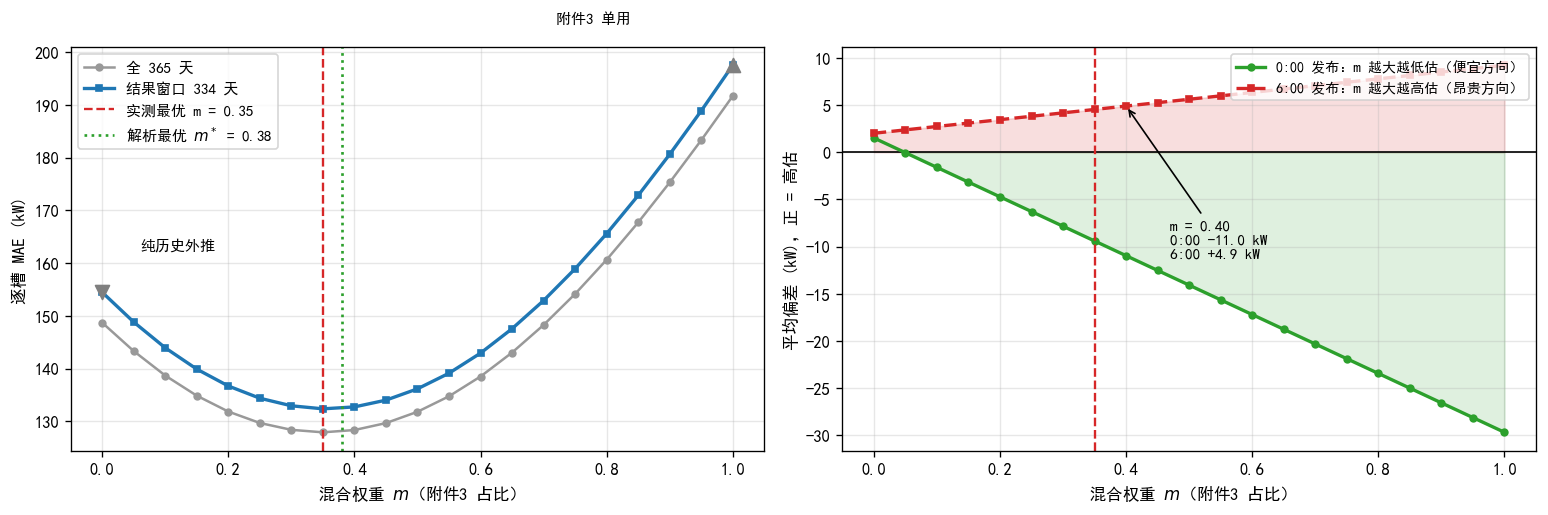
\includegraphics[width=0.95\textwidth]{光伏混合权重标定.png}
\caption{光伏混合权重的标定。(a) MAE 随 $m$ 的扫描曲线（两个统计窗口）：实测最优 $m=0.35\sim0.40$ 与解析最优 $m^{*}=0.38\sim0.40$ 重合；(b) 逐决策时刻的平均偏差（正 = 高估）：$m$ 增大时 0:00 发布的一版越来越\textbf{低估}（便宜方向），而 6:00 发布的一版越来越\textbf{高估}（昂贵方向），两者方向相反}
\label{fig:mix}
\end{figure}

\subsection{报童模型：两阶段的不同临界分位}
与问题二不同，问题三的两个阶段具有不同的边际成本结构。
\noindent\textbf{(a) 计划阶段（0:00）：}多买 1 kWh 多付 $\pi_t$；少买 1 kWh 则需按 $5\pi_t$ 紧急补足，净损失 $5\pi_t-\pi_t=4\pi_t$。故
\begin{equation}
    c_o=\pi_t,\quad c_u=4\pi_t,\qquad \alpha^{*}_p=\frac{c_u}{c_u+c_o}=\frac{4}{5}=0.80 .
\end{equation}
\noindent\textbf{(b) 调整阶段（6:00/12:00/18:00）：}相对计划量，多买 1 kWh 需付 $1.5\pi_t$；少买 1 kWh 虽退回 $0.5\pi_t$，但缺口仍按 $5\pi_t$ 补，故相对基线的净损失为 $5\pi_t-1.5\pi_t=3.5\pi_t$。于是
\begin{equation}
    c_o=1.5\pi_t,\quad c_u=3.5\pi_t,\qquad \alpha^{*}_a=\frac{c_u}{c_u+c_o}=\frac{3.5}{5}=0.70 .
\end{equation}
两个阶段共用同一裕量，故最优分位应落在 $[0.70,0.80]$，本文取中点 $\alpha^{*}=0.75$。误差样本取\textbf{负载}预报误差（问题三的光伏已由附件 3 承担，若再把光伏误差计入裕量，等于对同一不确定性重复设防）：
\begin{equation}
    \varepsilon_{j,t}=L^{\mathrm{real}}_{j,t}-\hat L_{j,t},\qquad
    X_{d,t}=\mathrm{Quantile}_{0.75}\bigl(\{\varepsilon_{j,t}\mid \max(0,d-W)\le j<d\}\bigr),\ W=60 .
\end{equation}

\noindent\textbf{误差口径的对照实验.}上述“避免重复设防”的理由是否成立，本文做了直接检验（\texttt{q3\_裕量误差口径.txt}）：在其余参数完全相同的条件下，只把误差定义换成净负荷误差 $(L-G)-(\hat L-\hat G)$，则同一分位（0.75）可省 10\,456.6 元（0.077\%），其最优分位组合（0.70）可省 19\,171.7 元（0.14\%）；而分位取 0.80 时会反而多付 84\,196.1 元。可见两种口径的差异在\textbf{噪声量级}（$\le0.14\%$），并不存在一方压倒性更优；本文保留负载误差口径，一是形式更简洁并与问题二可直接类比，二是它不随光伏预报方法的改变而漂移（稳健性更好）。

\textbf{裕量的敏感性.}全年费用关于分位数的曲线是平坦的（$\alpha^{*}=0.70$：13\,624\,983.0 元；0.75：\textbf{13\,589\,362.4} 元；0.80：13\,598\,164.7 元；0.85：13\,668\,602.1 元；0.90：13\,853\,989.1 元），与先验预测的 $[0.70,0.80]$ 区间吻合。作为对照，固定 300 kW 均匀裕量的全年费用为 13\,847\,475.1 元，本方案比它省 25.8 万元（1.86\%）；若完全不设裕量则为 14\,152\,041.6 元，本方案省 56.3 万元（3.98\%）。

\begin{figure}[htbp]
\centering
\begin{minipage}[c]{0.48\textwidth}
    \centering
    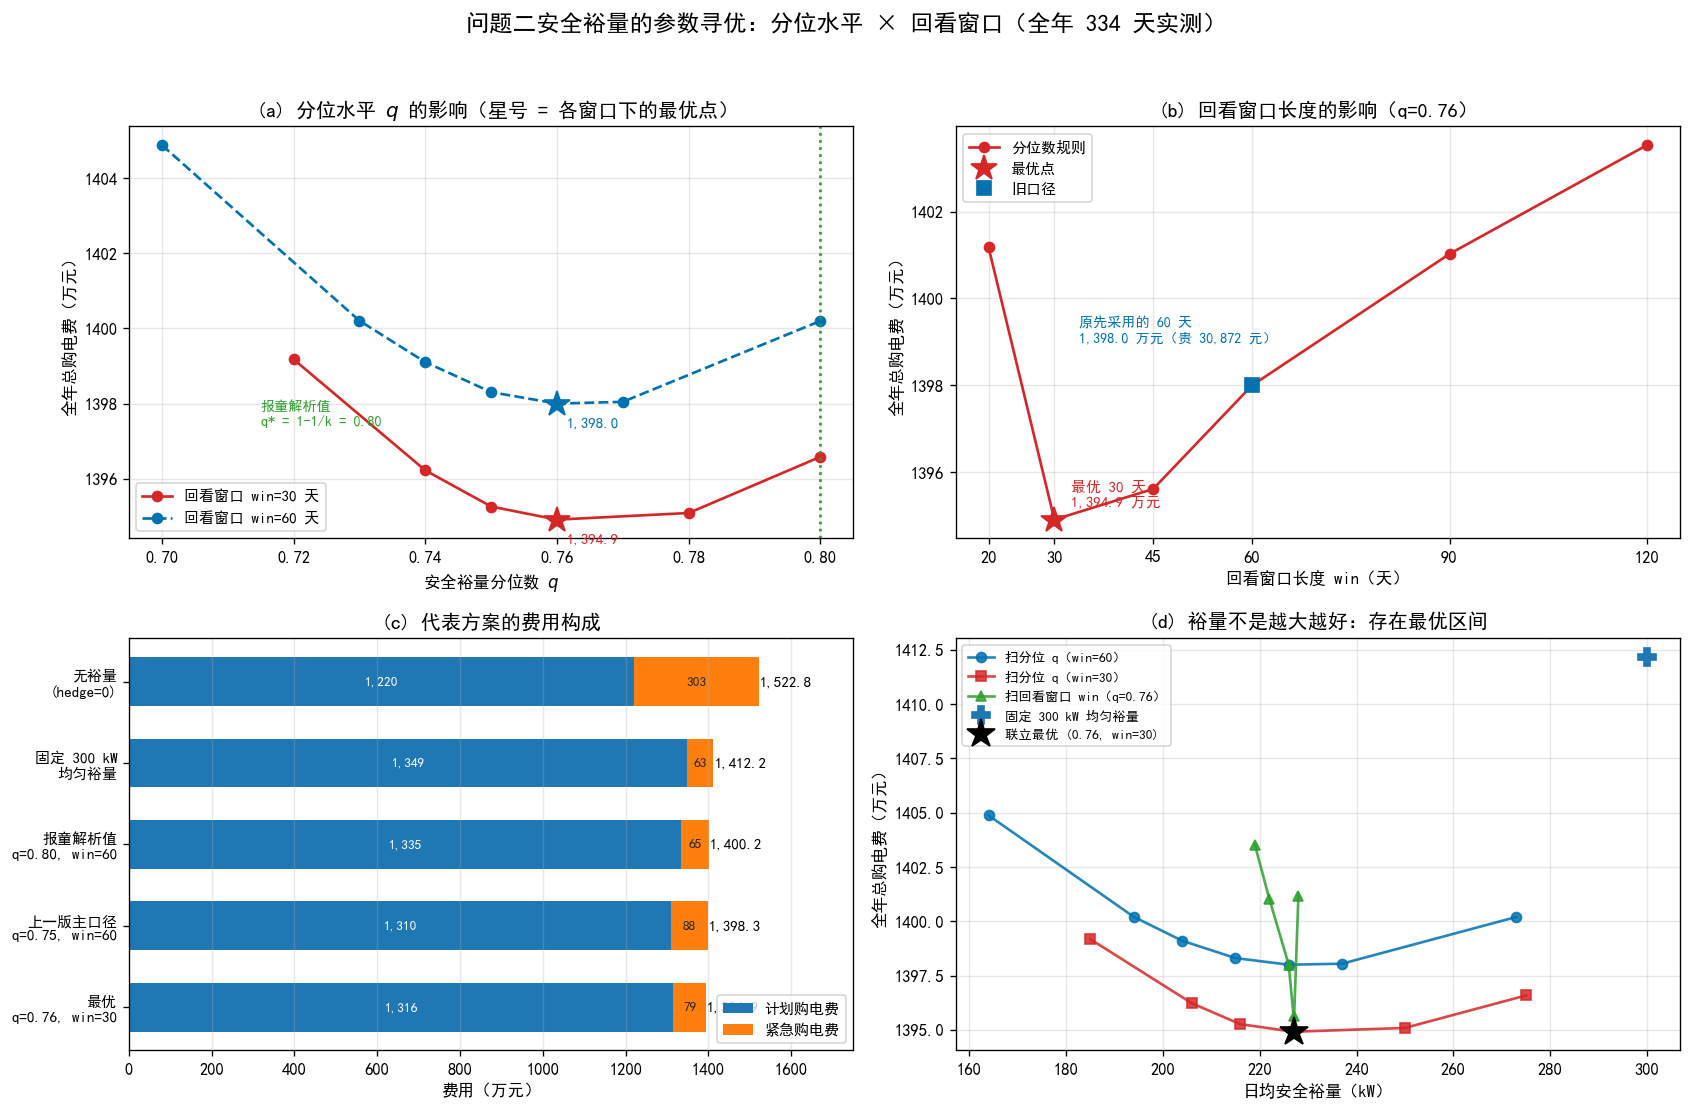
\includegraphics[width=\textwidth]{问题二裕量寻优.png}
    \subcaption{问题二：分位数 × 窗口寻优}
\end{minipage}\hfill
\begin{minipage}[c]{0.48\textwidth}
    \centering
    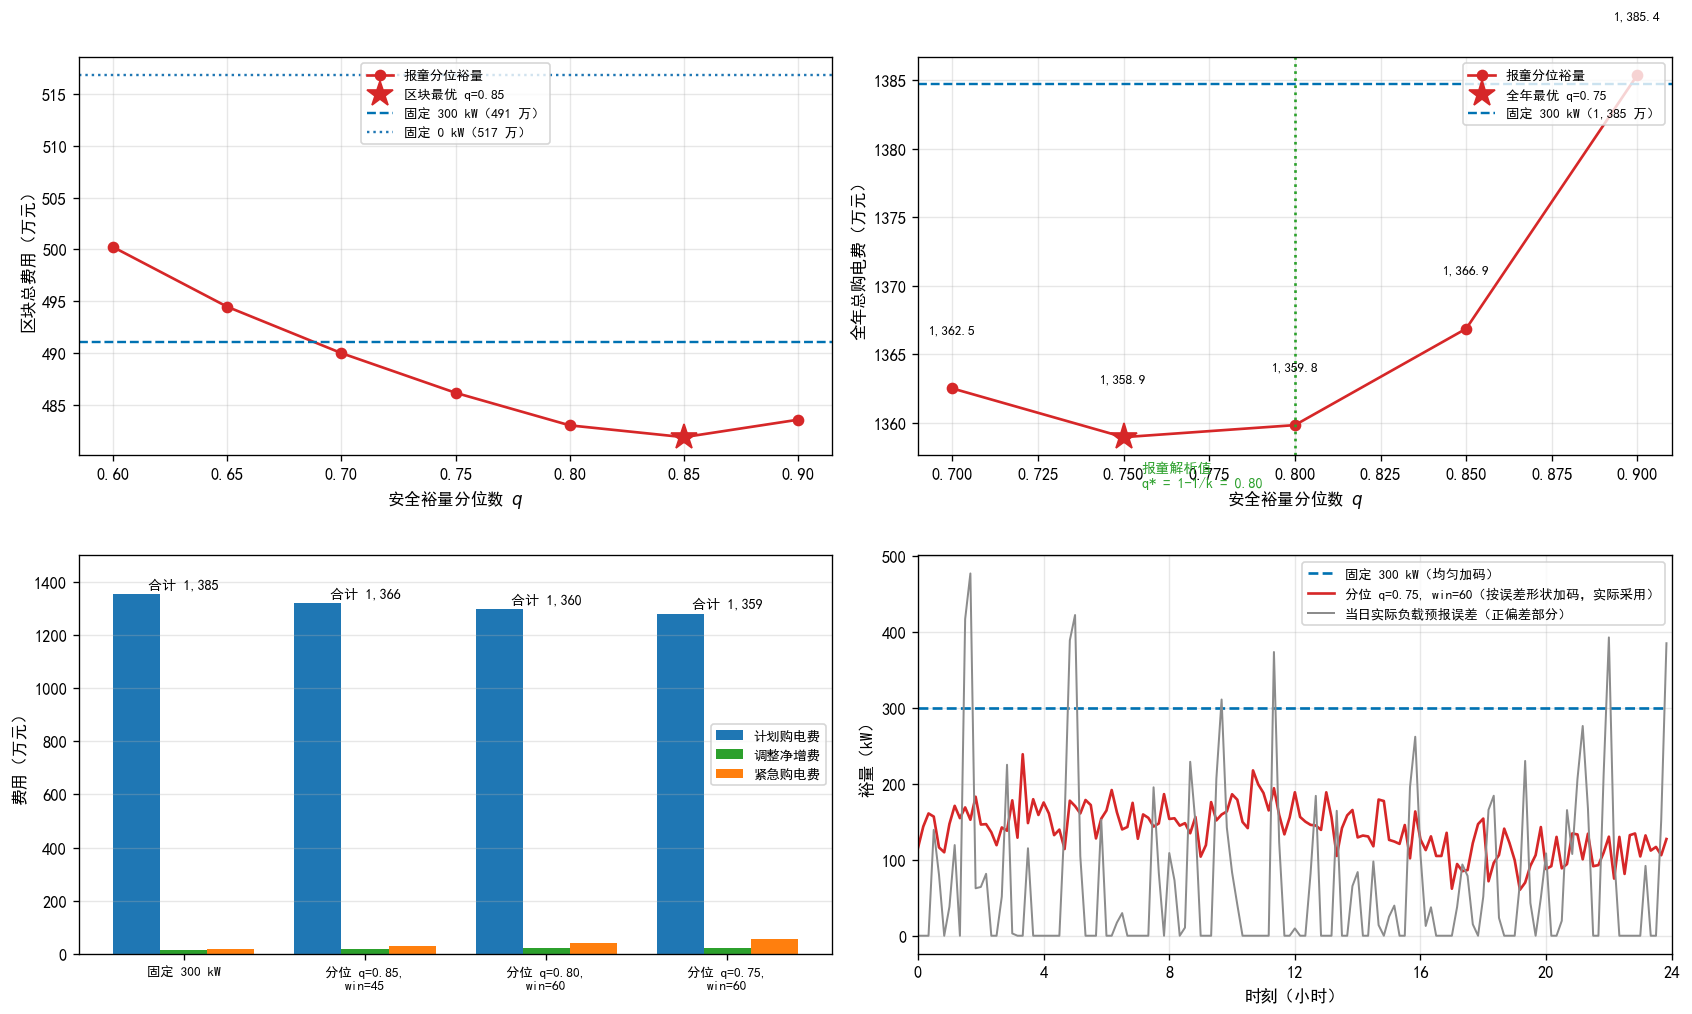
\includegraphics[width=\textwidth]{问题三裕量灵敏度.png}
    \subcaption{问题三：裕量灵敏度曲线}
\end{minipage}
\caption{报童裕量的参数寻优与灵敏度}
\end{figure}

\subsection{逐槽规则的精确 LP 嵌入}
问题三的调整阶段要同时决定购电量与储能动作。若把“逐槽被动平衡规则”写成仿真、再与 LP 交替迭代，既慢又可能出现前后矛盾。本文证明该规则本身是凸分段线性的，可用纯 LP 精确表达，从而\textbf{单层 LP 一步求解}。

在调整 LP 中，对 $t\ge t_0$：
\begin{align}
    \min\quad & \sum_{t\ge t_0}\Bigl[1.5\pi_t\delta^{+}_t-0.5\pi_t\delta^{-}_t+5\pi_t e_t+\epsilon s_t\Bigr]\Delta t \\
    \text{s.t.}\quad
    & b_t=b^p_t+\delta^{+}_t-\delta^{-}_t, \nonumber\\
    & d_t-c_t-s_t-e_t=L^{\mathrm f}_t-G^{\mathrm f}_t-b_t, \nonumber\\
    & d_t\le P_{\max},\qquad d_t\le (E_{t-1}-E_{\min})\eta/\Delta t, \nonumber\\
    & c_t\le P_{\max},\qquad c_t\le (E_{\max}-E_{t-1})/(\eta\Delta t), \nonumber\\
    & s_t\le G^{\mathrm f}_t,\qquad E_t=E_{t-1}+(\eta c_t-d_t/\eta)\Delta t,\quad E_t\in[E_{\min},E_{\max}], \nonumber\\
    & b_t,\delta^{\pm}_t,c_t,d_t,s_t,e_t\ge0. \nonumber
\end{align}

\textbf{为什么等价.} 目标中 $e_t$ 的系数 $5\pi_t>0$ 会迫使放电 $d_t$ 取到上界
\[
    d_t=\min\Bigl(\Delta_t,\ P_{\max},\ \frac{(E_{t-1}-E_{\min})\eta}{\Delta t}\Bigr);
\]
$s_t$ 的系数取极小正值 $\epsilon=10^{-6}$ 会迫使充电 $c_t$ 取到上界
\[
    c_t=\min\Bigl(-\Delta_t,\ P_{\max},\ \frac{E_{\max}-E_{t-1}}{\eta\,\Delta t}\Bigr).
\]
$\epsilon$ 只用于打破简并（弃光与充电在多解时的选择），不改变最优值。于是 LP 的最优解与逐槽规则的执行结果\textbf{逐点一致}。

\noindent\textbf{数值验证.}等价性对照必须对齐四个条件：\textbf{同一预报、同一安全裕量、LP 自己解出的购电量、同一入口 SOC}（缺任一条件都会人为制造虚假偏差）。在四者对齐后作三层比对：
（i）以 2025-03-20 为例，三个决策时刻的 $c_t,d_t,s_t,e_t,E_t$ 与逐槽规则的执行结果逐点偏差均 $\le7\times10^{-4}$（CBC 求解容差量级），见图 \ref{fig:q3_embed}(a)；
（ii）对全部 334 天作同样比对，\textbf{决定费用的两个量——购电量 $b$ 与紧急购电量 $e$——逐点一致}（$e$ 的最大逐点偏差 $5.5\times10^{-4}$ kWh，且三个决策时刻的合计均为 0）；
（iii）两解唯一可能不同的是 $c_t/d_t/s_t$ 的\textbf{分配}：LP 侧弃光比逐槽规则少 23.0 万 kWh（1\,588\,225.3 与 1\,818\,479.5 kWh），故两者目标函数之差仅为 $\epsilon\cdot\Delta(\text{弃光})=-0.23$ 元，相对 1360 万元总费用为 $10^{-8}$ 量级。
这说明差异属于\textbf{同一最优值下的破简并选择}（$\epsilon=10^{-6}$ 只是打破简并的极小系数），而不是“LP 假定了一个执行不了的解”：LP 挑出的 $b$ 可由逐槽规则物理执行，且执行后的紧急购电与 LP 的假设完全一致。

\noindent\textbf{自检.}上述单日复算同时给出了该日的表格值：全天调整购电量 67\,139.0151 kWh（表 1：67\,139.0151）、紧急购电 102.1300 kWh（表 3：102.1300）、24:00 储电量 1799.52 kWh（表 2：1799.52），三项均逐位一致，说明“模型—求解—执行—报表”四个环节共用同一套口径。

\begin{figure}[htbp]
\centering
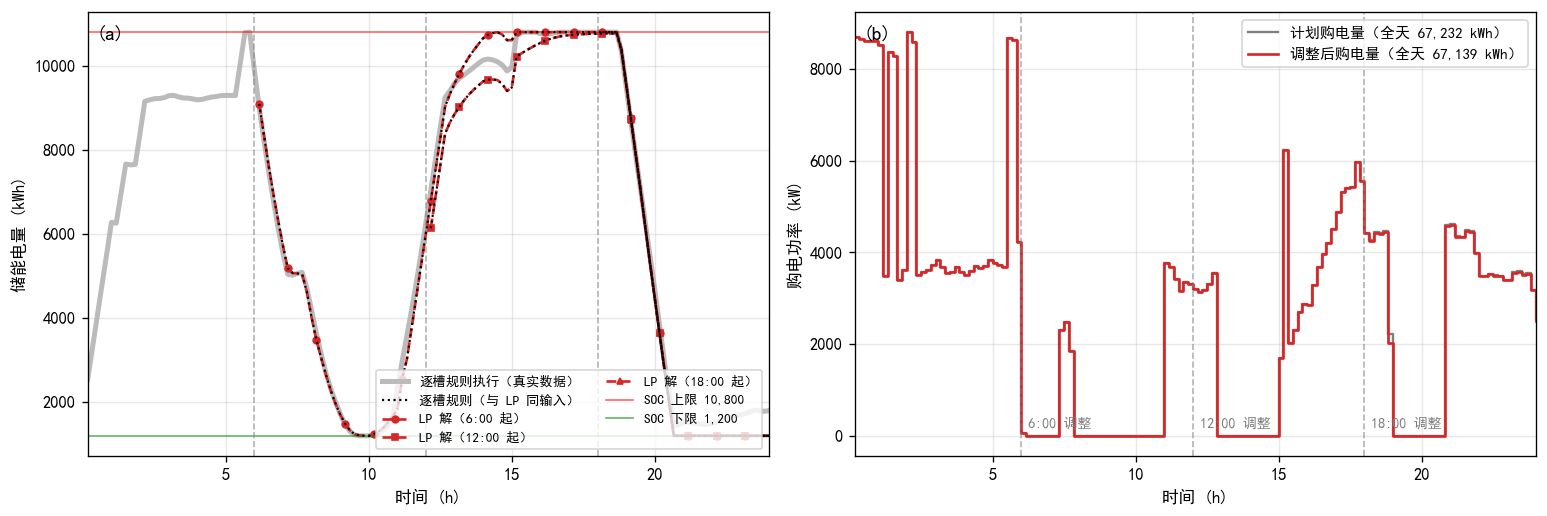
\includegraphics[width=0.96\textwidth]{fig_论文_问题三嵌入验证.png}
\caption{逐槽规则嵌入 LP 的等价性验证（2025-03-20）。(a) 在“同预报 $+$ 同裕量 $+$ LP 自解的购电量 $+$ 同入口 SOC”对齐后，LP 认为的 SOC（虚线）与逐槽规则执行的 SOC（点线）完全重合，逐点偏差 $<7\times10^{-5}$ kW；(b) 滚动调整在 6:00/12:00/18:00 对购电量曲线做出的修正}
\label{fig:q3_embed}
\end{figure}

\noindent\textbf{对照：把同一购电量放到实际数据下执行.}若把各决策时刻的 LP 解直接放到实际负载与光伏下执行（不再重新决策），将因预报误差产生紧急购电 100\,706.4 kWh（6:00）、66\,140.5 kWh（12:00）、19\,030.7 kWh（18:00）。需注意三者的统计区间依次嵌套（分别自 6:00、12:00、18:00 起算），故不可相加；该项与嵌入精度无关，正是预报误差的代价，与 8.7 节的完全信息下界互相印证。

\subsection{滚动逻辑的自洽性}
$t_0$ 时刻只优化 $t\in[t_0,144)$ 的购电量，$[0,t_0)$ 已发生、其费用为常数不影响 argmin；进入 $t_0$ 时的储电量由“实际数据 + 已锁定购电量”仿真得到，是已知量。又因逐槽规则无前瞻，“全天仿真 = 分段仿真拼接”，故滚动过程不会出现前后矛盾。此外，由于 $L_t$ 的预报误差只通过 $X_{d,t}$ 进入模型，而 $X$ 只用 $j<d$ 的样本，滚动过程不会使用未来信息。

\subsection{求解结果}
\begin{center}
\small
\begin{tabular}{lrlr}
\hline
指标 & 数值 & 指标 & 数值 \\
\hline
计划购电量 & 20\,897\,772.0 kWh & 计划购电费 & 12\,807\,426.8 元 \\
调整后购电量 & 20\,998\,542.4 kWh（净 $+$100\,770.5） & 调整相关购电费（含计划） & 13\,044\,668.0 元 \\
紧急购电量 & 102\,412.3 kWh（0.49\%） & 紧急购电费 & 544\,694.4 元 \\
\textbf{总购电费} & \textbf{13\,589\,362.4 元} & 发生调整的天数 & 334 / 334 天 \\
充电量 & 6\,420\,546.4 kWh & 放电量 & 5\,201\,470.9 kWh \\
弃光量 & 1\,942\,689.7 kWh & 出现紧急购电天数 & 153 / 334 天 \\
\hline
\end{tabular}
\end{center}

相对问题二，问题三的总购电费下降 359\,746.1 元（2.58\%），且紧急购电量由 141\,988.6 kWh 降至 102\,412.3 kWh（降 27.9\%）。这说明“允许滚动调整 + 双向惩罚”的组合是有利的：虽然调整本身要付 0.5$\sim$1.5 倍电价的偏差费（全年净增 237\,241.2 元），但它让储能得以在正确的时段充放电，从而省下更多的紧急购电费与峰段购电费，净效果为负。

\noindent\textbf{完美信息下界.}若 0:00 即准确知道当天全部实际负载与光伏，则 0:00 的计划 LP 即为全天确定性最优解，此时任何后续调整都无法改进（否则与原解最优性矛盾），故必有 $b^a=b^p$、$\delta^{\pm}=0$、$e=0$。实测：调整段与计划段的购电量最大偏差 $1.0\times10^{-5}$ kW，紧急购电量 0.0007 kWh（浮点噪声），全年费用为 \textbf{12\,254\,765.7 元}。于是预报误差的代价（完全信息价值）为
\begin{equation}
    13\,589\,362.4-12\,254\,765.7=1\,334\,596.7\ \text{元}\ (9.82\%).
\end{equation}
这一数字给出了预报与裕量改进的天花板：即使把预报做到零误差，全年最多再省 133.5 万元。值得注意的是，完美信息下\textbf{弃光量由 194.3 万 kWh 降至 99.0 万 kWh}，即预报误差的伤害是双重的——它既推高紧急购电，又让储能“充错时段”，使本该吸纳的光伏被弃掉。

\begin{figure}[htbp]
\centering
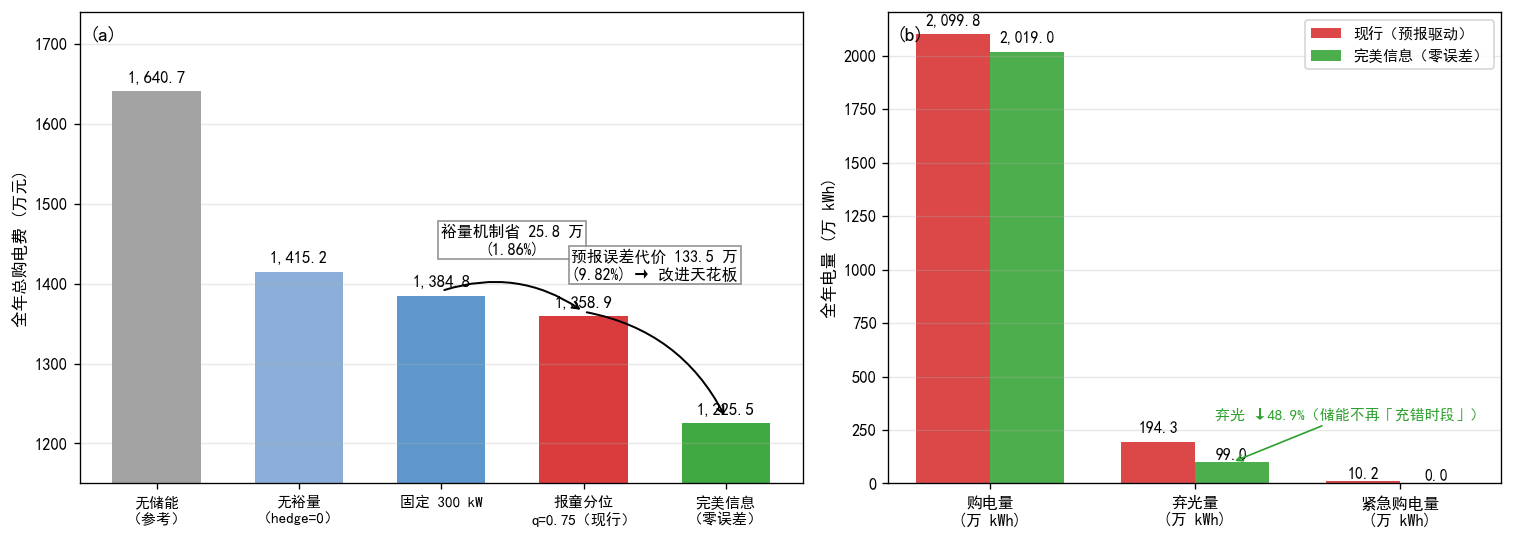
\includegraphics[width=0.96\textwidth]{fig_论文_问题三完美信息.png}
\caption{问题三的价值阶梯与结构对比。(a) 无储能 1640.7 万元 $\to$ 无裕量 1415.2 $\to$ 固定 300 kW 1384.7 $\to$ 现行（报童分位 0.75）1358.9 $\to$ 完美信息 1225.5 万元：裕量机制值 25.8 万元，预报误差代价 133.5 万元；(b) 完美信息下弃光量下降 48.9\%、紧急购电归零}
\label{fig:q3_perfect}
\end{figure}

\begin{table}[htbp]
\centering
\caption{\textbf{微网在指定时间段的购电量及全天购电量、购电费（问题三，单位：kWh / 元）}}
\label{tab:q3_buy}
\adjustbox{max width=\textwidth}{%
\begin{tabular}{|c|c|c|c|c|c|c|c|c|}
\hline
\multirow{2}{*}{时间段} & \multicolumn{2}{c|}{2025.3.20} & \multicolumn{2}{c|}{2025.6.21} & \multicolumn{2}{c|}{2025.9.23} & \multicolumn{2}{c|}{2025.12.21} \\
\cline{2-9}
 & 计划 & 调整 & 计划 & 调整 & 计划 & 调整 & 计划 & 调整 \\
\hline
10:00-10:10 & 0.0000 & 0.0000 & 0.0000 & 0.0000 & 0.0000 & 0.0000 & 0.0000 & 0.0000 \\
\hline
12:00-12:10 & 521.2658 & 521.2658 & 0.0000 & 0.0000 & 406.1960 & 406.1960 & 929.3245 & 929.3245 \\
\hline
14:00-14:10 & 0.0000 & 0.0000 & 0.0000 & 0.0000 & 0.0000 & 0.0000 & 0.0000 & 0.0000 \\
\hline
16:00-16:10 & 546.6403 & 546.6403 & 211.3272 & 211.3272 & 571.0562 & 571.0562 & 814.4589 & 814.4589 \\
\hline
18:00-18:10 & 709.9800 & 707.2799 & 0.0000 & 0.0000 & 772.1585 & 768.5508 & 745.5538 & 745.0377 \\
\hline
20:00-20:10 & 0.0000 & 0.0000 & 0.0000 & 0.0000 & 0.0000 & 0.0000 & 0.0000 & 0.0000 \\
\hline
全天购电量 & 67\,231.5478 & 67\,139.0151 & 35\,068.8637 & 35\,225.3443 & 67\,981.2421 & 67\,856.0386 & 96\,126.8105 & 96\,109.5646 \\
\hline
全天购电费 & 41\,015.6293 & 40\,971.4454 & 20\,853.6060 & 21\,154.1831 & 42\,511.0031 & 42\,450.2266 & 61\,868.6481 & 61\,860.4725 \\
\hline
\end{tabular}
}
\end{table}

\begin{table}[htbp]
\centering
\caption{\textbf{储能设备在指定时间段的充放电量及 0:00 与 24:00 的储电量（问题三，单位：kWh）}}
\label{tab:q3_soc}
\adjustbox{max width=\textwidth}{%
\begin{tabular}{|c|c|c|c|c|c|c|c|c|}
\hline
\multirow{2}{*}{时间段} & \multicolumn{2}{c|}{2025.3.20} & \multicolumn{2}{c|}{2025.6.21} & \multicolumn{2}{c|}{2025.9.23} & \multicolumn{2}{c|}{2025.12.21} \\
\cline{2-9}
 & 充电量 & 放电量 & 充电量 & 放电量 & 充电量 & 放电量 & 充电量 & 放电量 \\
\hline
0:00-4:00   & 8\,391.43 & 132.87   & 701.77 & 94.77    & 8\,473.87 & 17.44    & 8\,694.86 & 153.43 \\
\hline
4:00-8:00   & 1\,865.03 & 6\,027.72 & 915.80 & 1\,751.64 & 1\,384.16 & 6\,663.87 & 2\,402.28 & 1\,527.44 \\
\hline
8:00-12:00  & 5\,652.02 & 2\,675.25 & 9\,396.15 & 0.00  & 5\,136.20 & 1\,896.62 & 5\,503.83 & 7\,186.66 \\
\hline
12:00-16:00 & 5\,329.12 & 287.26   & 0.00 & 0.00    & 5\,924.91 & 494.58   & 7\,261.71 & 2\,320.09 \\
\hline
16:00-20:00 & 63.58 & 5\,527.01    & 252.02 & 5\,157.72 & 100.76 & 5\,652.30    & 0.00 & 5\,658.23 \\
\hline
20:00-24:00 & 503.06 & 2\,999.86   & 1\,319.78 & 2\,485.90 & 713.72 & 3\,078.02 & 555.03 & 2\,863.28 \\
\hline
0:00 储电量  & \multicolumn{2}{c|}{1\,786.79} & \multicolumn{2}{c|}{2\,939.21} & \multicolumn{2}{c|}{2\,025.83} & \multicolumn{2}{c|}{1\,754.29} \\
\hline
24:00 储电量 & \multicolumn{2}{c|}{1\,799.52} & \multicolumn{2}{c|}{3\,721.71} & \multicolumn{2}{c|}{1\,805.18} & \multicolumn{2}{c|}{1\,831.18} \\
\hline
\end{tabular}
}
\end{table}

\begin{table}[htbp]
\centering
\caption{\textbf{微网在指定日期的紧急购电量（问题三，单位：kWh）}}
\label{tab:q3_emg}
\begin{tabular}{|c|c|c|c|c|}
\hline
时间段 & 2025.3.20 & 2025.6.21 & 2025.9.23 & 2025.12.21 \\
\hline
0:00-4:00   & 0.0000 & 0.0000 & 0.0000 & 0.0000 \\
\hline
4:00-8:00   & 0.0000 & 0.0000 & 0.0000 & 23.8278 \\
\hline
8:00-12:00  & 102.1300 & 0.0000 & 0.0000 & 0.0000 \\
\hline
12:00-16:00 & 0.0000 & 0.0000 & 0.0000 & 0.0000 \\
\hline
16:00-20:00 & 0.0000 & 0.0000 & 0.0000 & 0.0000 \\
\hline
20:00-24:00 & 0.0000 & 0.0000 & 6.3750 & 0.0000 \\
\hline
全天合计 & 102.1300 & 0.0000 & 6.3750 & 23.8278 \\
\hline
\end{tabular}
\end{table}

\subsection{结果分析}
与问题二相比，问题三的调整幅度总体很小（四个日期的全天购电量变化均在 $-0.15\%$ 以内），但对个别时段的修正很关键：例如 2025-09-23 的 $18{:}00\sim18{:}10$ 由计划的 772.16 kWh 下调至 768.55 kWh，避免了在晚峰为多余电量支付违约费；2025-03-20 的紧急购电由问题二的 209.62 kWh（$20{:}20\sim21{:}30$）变为 102.13 kWh（$8{:}00\sim12{:}00$），说明 6:00 与 12:00 的两次光伏预报更新修正了原先被低估的日间缺口。春季、秋季、冬季三天的储能均在凌晨谷段大量充电（约 8\,400$\sim$8\,700 kWh），夏季因光伏充足而充电主要集中在 $8{:}00\sim12{:}00$。

\section{问题四模型的建立与求解}
\subsection{模型建立}
问题四把固定电价换成附件 4 的逐日波动电价。因电价曲线由日前市场提前公布，0:00 即可获知当天完整的 144 个时段价格，故电价\textbf{无需预测}，直接把目标函数与结算价中的 $\pi_t$ 替换为当天的实际电价即可，其余模型结构、预测方法与裕量口径与问题二/三完全一致。这构成了一个天然受控实验：同一模型、同一预测、仅换电价。

附件 4 的电价特征为：全局 $0.0076\sim1.7936$ 元/kWh，均值 0.7662 元/kWh（与附件 1 相同）；逐日均价在 $0.5378\sim0.9290$ 之间漂移（标准差 0.1036）；日内峰谷比均值 5.74，明显高于附件 1 的 3.76。

\subsection{求解结果}
\begin{center}
\small
\begin{tabular}{lrrr}
\hline
口径 & 固定电价（附件 1） & 波动电价（附件 4） & 变化 \\
\hline
对应问题二（元） & 13\,949\,108.5 & 14\,634\,080.5 & $+$4.91\% \\
对应问题三（元） & 13\,589\,362.4 & 14\,210\,954.8 & $+$4.57\% \\
计划购电量（kWh） & --- & 21\,505\,541.3 / 20\,969\,438.2 & --- \\
紧急购电量（kWh） & --- & 146\,514.8 / 98\,327.5 & --- \\
实际平均单价（元/kWh） & 0.6505 & 0.6805 & $+$4.61\% \\
无储能参考（元） & 16\,407\,319.6 & 17\,026\,782.9 & $+$3.78\% \\
\hline
\end{tabular}
\end{center}
（“对应问题二/三”两行分别为问题四沿用问题二、问题三口径重算的全年费用；计划购电量与紧急购电量两行为“问题二口径 / 问题三口径”。）

\subsection{涨价机理的受控分解}
一个容易产生的误解是“电价峰谷比变大 ⇒ 储能套利空间变大”。但事实上：波动电价下统计窗口内的\textbf{均价更低}（0.7575 元/kWh $<$ 0.7662 元/kWh），费用却更高。为定位原因，本文做如下受控分解：以问题二的固定电价最优策略为基准，逐步替换为附件 4 的电价。

\begin{center}
\begin{tabular}{lrl}
\hline
分解项 & 金额（元） & 占比 \\
\hline
逐时段均价项（把每个时段的价格换成窗口均值） & $+$16\,966.3 & 2.8\% \\
逐日漂移项（每天的均价相对窗口均价的偏离） & $+$585\,294.0 & 97.2\% \\
合计（计划购电费增量） & $+$602\,260.3 & 100\% \\
\hline
\end{tabular}
\end{center}

逐日漂移项贡献了 97.2\% 的增量。进一步检验其机制：日购电量与当日电价水平的相关系数为 $+0.9651$——高负载日恰好也是高电价日，而储能容量（12000 kWh，可用 9600 kWh）远小于单日购电量（约 6.4 万 kWh），根本无法跨日套利。也就是说，波动电价带来的额外成本无法通过“日内套利”消除，只能通过“更贴合当日曲线地安排充放电”部分缓解，这正是问题三口径（滚动调整）比问题二口径（固定计划）涨价更少（4.57\% $<$ 4.91\%）的原因。

作为交叉验证：把问题二得到的策略直接放到附件 4 的电价下结算（即“A 的方案、B 的价格”）需要 13\,883\,703.9 元，而问题四重新优化后为 13\,757\,329.3 元，LP 通过重新调度节省了 126\,374.6 元，说明模型对电价变化确实做出了有效响应。

\begin{figure}[htbp]
\centering
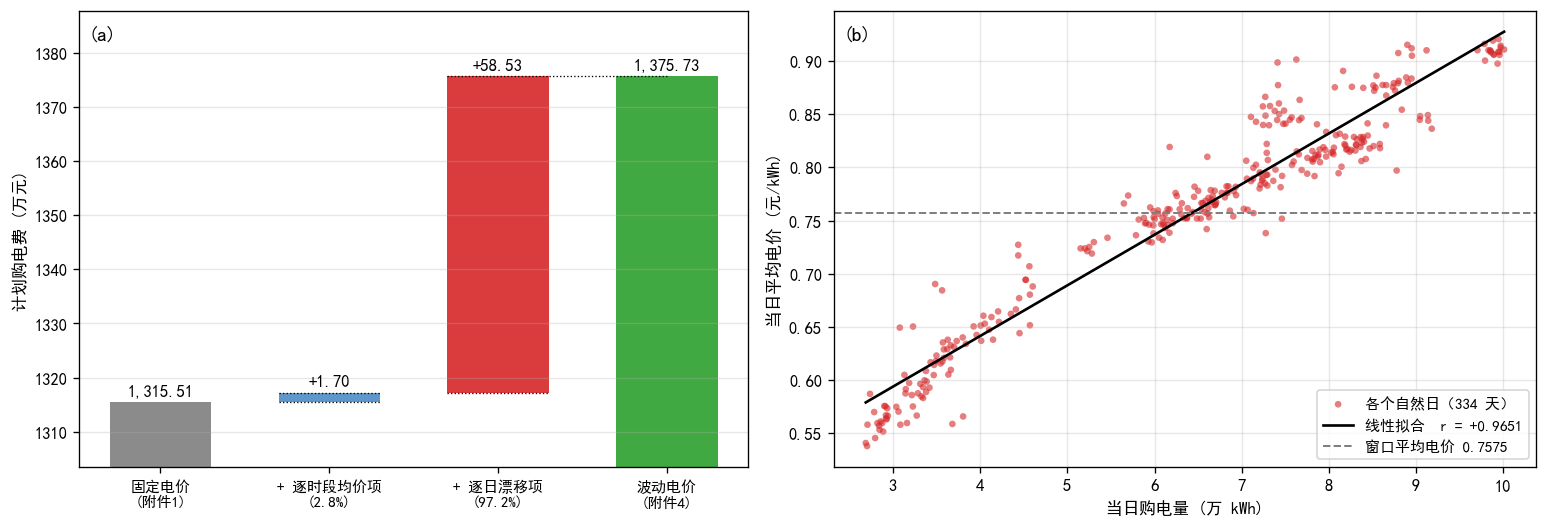
\includegraphics[width=0.96\textwidth]{fig_论文_问题四涨价机理.png}
\caption{电价波动的影响分解。(a) 计划购电费由 1315.5 万元升至 1375.7 万元，其中逐时段均价项仅贡献 2.8\%（且窗口均价 0.7575 低于附件 1 的 0.7662），97.2\% 来自逐日电价漂移；(b) 日购电量与当日电价水平的相关系数达 $+0.9651$，高负载日恰为高电价日，而储能可用容量仅 9600 kWh，无法跨日套利}
\label{fig:q4_mech}
\end{figure}

\subsection{指定日期的结果}
\begin{table}[htbp]
\centering
\caption{\textbf{波动电价下微网在指定时间段的购电量（问题四，单位：kWh）}}
\label{tab:q4_buy}
\adjustbox{max width=\textwidth}{%
\begin{tabular}{|c|c|c|c|c|c|c|c|c|c|}
\hline
时间段 & 3.20（二口径） & 3.20（三口径） & 6.21（二口径） & 6.21（三口径） & 9.23（二口径） & 9.23（三口径） & 12.21（二口径） & 12.21（三口径） \\
\hline
10:00-10:10 & 0.00 & 0.00 & 0.00 & 0.00 & 0.00 & 0.00 & 0.00 & 0.00 \\
\hline
12:00-12:10 & 517.65 & 521.27 & 0.00 & 0.00 & 492.71 & 406.20 & 949.98 & 929.32 \\
\hline
14:00-14:10 & 0.00 & 0.00 & 0.00 & 0.00 & 0.00 & 0.00 & 0.00 & 0.00 \\
\hline
16:00-16:10 & 482.80 & 546.64 & 251.37 & 211.33 & 572.00 & 571.06 & 832.47 & 814.46 \\
\hline
18:00-18:10 & 0.00 & 0.00 & 504.40 & 551.12 & 0.00 & 0.00 & 739.25 & 745.04 \\
\hline
20:00-20:10 & 0.00 & 0.00 & 0.00 & 0.00 & 803.27 & 798.35 & 0.00 & 0.00 \\
\hline
全天购电量 & 66\,448.56 & 67\,414.78 & 36\,633.19 & 35\,864.35 & 69\,314.94 & 67\,658.86 & 98\,532.56 & 96\,004.39 \\
\hline
全天购电费 & 41\,320.85 & 41\,876.79 & 18\,523.67 & 18\,237.86 & 44\,390.54 & 43\,657.40 & 74\,750.04 & 72\,330.52 \\
\hline
\end{tabular}
}
\end{table}

\begin{table}[htbp]
\centering
\caption{\textbf{波动电价下微网在指定日期的紧急购电量（问题四，单位：kWh）}}
\label{tab:q4_emg}
\small
\begin{tabular}{|c|c|c|l|}
\hline
日期 & 问题二口径 & 问题三口径 & 说明 \\
\hline
2025.3.20 & 0.00 & 102.29 & 三口径在上午出现缺口 \\
\hline
2025.6.21 & 0.00 & 0.00 & 光伏充足，无缺口 \\
\hline
2025.9.23 & 209.62 & 7.46 ($1.08+6.38$) & 晚峰电价更高，二口径缺口更大 \\
\hline
2025.12.21 & 0.00 & 23.83 & 晨峰价格高，三口径出现小额缺口 \\
\hline
\end{tabular}
\end{table}

\subsection{结果分析}
波动电价下，购电时段的分布发生了可见的迁移：2025-03-20 与 2025-06-21 的 $18{:}00\sim18{:}10$ 购电量由固定电价下的 713.46 / 0.00 kWh 变为 0.00 / 504.40 kWh，说明模型把购电从当日的高价时段挪到了低价时段；2025-09-23 的 $20{:}00\sim20{:}10$ 由 0.00 增至 803.27 kWh，则是由于该日 $12{:}00$ 与 $18{:}00$ 相对更便宜，模型选择在这些时段多买、以降低晚峰缺口。这正是“电价曲线每天都不同”对策略的真实影响。

\section{灵敏度与稳健性分析}
本节对每个问题的关键参数逐一扰动。所有比较都落在同一个最终指标上——\textbf{全年购电费用}
（结果窗口 2025-02-01 起 334 天），以保证不同参数之间可比。所用脚本与原始输出
（\texttt{q2\_敏感性分析.txt}、\texttt{q2\_裕量精细寻优.txt}、\texttt{q2\_裕量稳健性检验.txt}、
\texttt{q2\_光伏预报方法.txt}、\texttt{q3\_裕量灵敏度.txt} 等）均随交付文件提供。

\subsection{问题二：预测精度、紧急电价倍率与安全裕量}
问题二的建模链条上有两个来自题面的假设（日前预报的精度、紧急购电按 5 倍电价结算）
与一个由本文自己选定的参数（安全裕量）。下面依次扰动这三者，检验结论是否稳健（汇总见图 \ref{fig:q2_sens}）。

\subsubsection{预测精度：费用的增长几乎全部由紧急购电承担}
为量化“预报准一点究竟能省多少钱”，构造一族反事实预报序列，把预报误差整体缩放 $\lambda$ 倍：
\begin{equation}
    \hat F' = y + \lambda\left(\hat F - y\right),
    \label{eq:lam}
\end{equation}
其中 $y$ 为实际值、$\hat F$ 为本文实测口径（负载 wday:7、光伏 ma:3）的预报：$\lambda=0$ 表示完美预测，
$\lambda=1$ 是实测口径，$\lambda>1$ 表示预报更差。为隔离“预报精度”这一个因素，
本实验全程固定使用 300 kW 均匀裕量（不用分位数裕量）。

\begin{table}[htbp]
\centering
\caption{预报误差缩放 $\lambda$ 对全年费用与风险敞口的影响（334 天，裕量固定 300 kW）}
\label{tab:q2_sens_lam}
\begin{adjustbox}{max width=\textwidth}
\begin{tabular}{ccccccc}
\hline
$\lambda$ & 净负荷误差 MAE (kW) & 计划购电费 (元) & 紧急购电量 (kWh) & 紧急购电费 (元) & 总购电费 (元) & 有紧急购电的天数 \\
\hline
0.0 & 0.0 & 13\,514\,290.5 & 0.0 & 0.0 & 13\,514\,290.5 & 0/334 \\
0.5 & 138.3 & 13\,495\,677.5 & 12\,171.3 & 75\,075.6 & 13\,570\,753.1 & 25/334 \\
1.0 & 276.7 & 13\,488\,522.9 & 112\,059.1 & 633\,131.1 & 14\,121\,654.0 & 85/334 \\
1.5 & 415.0 & 13\,497\,462.3 & 256\,686.4 & 1\,442\,177.2 & 14\,939\,639.5 & 128/334 \\
2.0 & 553.4 & 13\,529\,657.1 & 406\,481.1 & 2\,250\,217.0 & 15\,779\,874.0 & 147/334 \\
\hline
\end{tabular}
\end{adjustbox}
\end{table}

\noindent 表 \ref{tab:q2_sens_lam} 给出三点结论。\textbf{第一，实验本身是干净的：}
MAE 严格随 $\lambda$ 线性放大（$276.7\times0.5=138.3$、$276.7\times2=553.4$），
说明反事实序列只改变了误差幅度、没有引入别的差异。\textbf{第二，计划购电费几乎与预报精度无关：}
五个 $\lambda$ 下计划购电费的极差只有 41\,134.2 元（0.30\%），费用的全部增长都发生在紧急购电侧。
$\lambda$ 由 1 增加到 2 时总费用上升 1\,658\,220.0 元（$+11.7\%$），
其中 1\,617\,085.9 元（97.5\%）是紧急购电费。这说明日前计划买多少电这件事本身是“稳”的，
真正的风险来自\textbf{计划之外被迫临时买贵电}。\textbf{第三，完美预测的价值有限但可观：}
$\lambda=0$ 相对实测口径仅省 607\,363.5 元（4.3\%）；与此同时“出现紧急购电”的天数
由 0 天膨胀到 147 天（$\lambda=2$ 时已占 44\%）。换言之，
预报误差带来的损失不是通过“让计划变差”实现的，而是通过“制造缺口并被迫按 5 倍价补上”实现的——
这恰好说明安全裕量必须针对\textbf{缺口的概率}设置，而不是针对误差的绝对值设置。

\subsubsection{报童模型的自检：最优裕量随误差幅度同比例放大}
报童模型的临界条件是“多买 1 kWh 的边际收益等于少买 1 kWh 的期望边际损失”，
即 $P(\text{缺口})>1/k$，它与误差的\emph{绝对幅度}无关，只与误差的\emph{分位数}有关。
因此若把误差整体放大 $\lambda$ 倍，最优裕量应当保持同一分位数、即近似放大 $\lambda$ 倍——
这是对报童建模思路的一个直接可证伪预言。在一个连续的 130 天区块（第 60$\sim$190 天）

\begin{table}[htbp]
\centering
\caption{误差幅度放大 $\lambda$ 倍时最优裕量的变化（130 天区块，单位：元）}
\label{tab:q2_sens_scale}
\begin{adjustbox}{max width=\textwidth}
\begin{tabular}{cccccc}
\hline
$\lambda$ & 净负荷误差 MAE (kW) & 裕量 0 kW & 裕量 300 kW & 裕量 600 kW & 区块最优裕量 \\
\hline
0.5 & 138.3 & 5\,079\,162 & 4\,787\,533 & 5\,216\,683 & 300 kW \\
1.0 & 276.7 & 5\,836\,835 & 5\,198\,549 & 5\,320\,603 & 300 kW \\
2.0 & 553.4 & 7\,090\,318 & 6\,187\,440 & 6\,058\,893 & 600 kW \\
\hline
\end{tabular}
\end{adjustbox}
\end{table}

\noindent 表 \ref{tab:q2_sens_scale} 中，误差幅度由 $\lambda=1$ 加倍到 $\lambda=2$ 时，
最优裕量由 300 kW 跳到 600 kW，方向与“分位数不变”的预言一致。但网格只有三档
（0 / 300 / 600 kW），$\lambda=0.5$ 与 $\lambda=1$ 都落在 300 kW 上，
故这只能算\textbf{一致性检验}，不足以宣称“严格线性”。此外该表还提供一个副产品：
$\lambda=1$ 时完全不设裕量（0 kW）的费用为 5\,836\,835 元，比设 300 kW 的 5\,198\,549 元
高出 638\,286 元（12.3\%），可见裕量并非可有可无的微调，而是费用结构中的主要杠杆。

\subsubsection{紧急电价倍率：惩罚强度是费用的一阶参数}
题面把紧急购电电价定为交易时刻电价的 5 倍。
把它换成 $k=3,4,5,6,8$ 五档，并同步按报童规则把裕量改为误差的 $(1-1/k)$ 分位数，
也就是让规则随 $k$ 自适应、而不是把裕量固定住：

\begin{table}[htbp]
\centering
\caption{紧急电价倍率 $k$ 的灵敏度（334 天，裕量按报童规则同步调整）}
\label{tab:q2_sens_k}
\begin{adjustbox}{max width=\textwidth}
\begin{tabular}{ccccccc}
\hline
$k$ & 理论分位 $1-1/k$ & 日均裕量 (kW) & 计划购电费 (元) & 紧急购电量 (kWh) & 紧急购电费 (元) & 总购电费 (元) \\
\hline
3 & 0.667 & 132 & 12\,759\,582.5 & 243\,215.2 & 833\,080.7 & 13\,592\,663.2 \\
4 & 0.750 & 215 & 13\,101\,901.1 & 158\,222.9 & 704\,909.9 & 13\,806\,811.0 \\
5 & 0.800 & 273 & 13\,347\,034.6 & 119\,752.3 & 654\,941.1 & 14\,001\,975.7 \\
6 & 0.833 & 318 & 13\,539\,066.0 & 98\,767.3 & 644\,078.8 & 14\,183\,144.8 \\
8 & 0.875 & 387 & 13\,834\,835.4 & 73\,972.8 & 643\,543.7 & 14\,478\,379.1 \\
\hline
\end{tabular}
\end{adjustbox}
\end{table}

\noindent 表 \ref{tab:q2_sens_k} 显示：$k$ 由 3 增至 8，总费用单调上升 885\,715.9 元（$+6.52\%$），
\textbf{说明“5 倍”这个惩罚强度本身就是费用的一阶参数}，而非无关紧要的题面细节。
更值得注意的是内部结构的变化：紧急购电费在 $k\ge6$ 之后基本饱和
（$k=6$ 为 644\,078.8 元，$k=8$ 为 643\,543.7 元，反而只降 535.1 元），
而计划购电费却一路从 12\,759\,582.5 元升到 13\,834\,835.4 元（$+8.43\%$）——
此时继续加大惩罚已不能减少缺口，只能逼迫模型在日前多买“保险电”，
其代价超过了省下的紧急购电费。这一“过犹不及”的拐点由模型自行给出，
对实际调度中如何设定违约电价有直接参考价值。
最后，按报童规则自适应地调整裕量，比“手工固定 300 kW”在同为 $k=5$ 时省 119\,678.3 元（0.85\%）——
\textbf{规则无需任何现场调参就能优于人工试凑的固定值}，这正是采用解析规则而非网格搜参的理由。

\subsubsection{安全裕量的 $(q,W)$ 规则：平坦谷底与分半稳健性}
裕量规则有两个参数：分位水平 $q$ 与误差回看窗口 $W$。先固定 $W=60$ 天细扫 $q$：

\begin{table}[htbp]
\centering
\caption{裕量分位 $q$ 与回看窗口 $W$ 的灵敏度（334 天）}
\label{tab:q2_sens_qw}
\begin{adjustbox}{max width=\textwidth}
\begin{tabular}{lcccc}
\hline
扫描方式 & 取值 & 日均裕量 (kW) & 全年总购电费 (元) & 相对本组最优点 \\
\hline
\multirow{4}{*}{固定 $W=60$，扫 $q$}
  & 0.70 & 164 & 14\,048\,781.9 & $+68\,801.3$（$+0.492\%$）\\
  & 0.75 & 215 & 13\,983\,038.5 & $+3\,058.0$（$+0.022\%$）\\
  & \textbf{0.76} & 226 & 13\,979\,980.5 & 最优点 \\
  & 0.80 & 273 & 14\,001\,975.7 & $+21\,995.2$（$+0.157\%$）\\
\hline
\multirow{5}{*}{固定 $q=0.76$，扫 $W$}
  & 20 天 & 228 & 14\,011\,828.8 & $+62\,720.3$（$+0.450\%$）\\
  & \textbf{30 天} & 227 & 13\,949\,108.5 & 最优点 \\
  & 45 天 & 227 & 13\,956\,168.8 & $+7\,060.3$（$+0.051\%$）\\
  & 60 天 & 226 & 13\,979\,980.5 & $+30\,872.0$（$+0.221\%$）\\
  & 120 天 & 219 & 14\,035\,321.8 & $+86\,213.2$（$+0.618\%$）\\
\hline
\multicolumn{2}{l}{固定 300 kW 均匀裕量} & 300 & 14\,121\,654.0 & 比 $q{=}0.76,W{=}30$ 贵 $172\,545.5$（$+1.237\%$）\\
\hline
\end{tabular}
\end{adjustbox}
\end{table}

\noindent 表 \ref{tab:q2_sens_qw} 有三层信息。
\textbf{(i) 解析值与实测最优值一致。}报童模型给出 $q^{*}=1-1/5=0.80$，
它与全年实测最优点 $q=0.76$ 的费用只差 21\,995.2 元（0.157\%），
且两者都明显优于固定裕量（14\,121\,654.0 元）。这说明\textbf{用解析规则定参是可靠的}，
而不必依赖全年数据做网格搜索——后者在只有 334 个样本时反而容易过拟合。
\textbf{(ii) 谷底是平的，不是尖的。}$q\in[0.73,0.80]$（固定 $W=60$）的极差为 0.158\%，
$W\in[30,120]$（固定 $q=0.76$）的极差为 0.618\%，都在 0.7\% 以内，
因此正确的表述是“$(q,W)$ 存在一片平坦的最优区域”，而不是“$q=0.76,W=30$ 是精确最优点”。
\textbf{(iii) 分半检验证明该参数没有过拟合风险。}把样本对半切开后，
上半年（167 天）的最优窗口是 30 天、下半年（167 天）的最优窗口是 45 天：
$W=30$ 相对 $W=60$ 在上半年省 39\,138.3 元（0.577\%），而在下半年反而贵 8\,318.9 元（0.116\%），
两者\textbf{方向不一致}。全年最优落在 30 天，只是因为上半年幅度大 5 倍而压过了下半年。
因此本文最终采用的 $(q,W)=(0.76,30)$ 应被理解为“处于平坦平台内”，
其 30\,872.0 元（0.221\%）的优势属于噪声量级，而非可移植的规律。
机制上也可解释：上半年（春夏）净负荷波动剧烈、误差水平变化快，短窗口跟得上；
下半年（秋冬）误差相对平稳，窗口长短关系不大（两半的极差 1.07\% 对 0.24\%）。

\subsubsection{预报方法本身的选择}
预报窗口 $k_w$ 的扫描见 7.2.2 节：MAE 最优在 $k_w=5$（151.5 kW）而全年费用最优在 $k_w=4$
（13\,939\,256.8 元），$k_w=3\sim7$ 构成平坦平台（费用极差 0.25\%），
$k_w=1$ 与 $k_w=10$ 分别劣化 0.69\% 与 0.40\%。作为极端对照，
若完全不用最近历史、改用附件 1 基准日的气候态曲线，费用将升至 14\,839\,836.8 元（$+6.39\%$），
说明“必须用最近的历史”这条结论与窗口长短无关。

\begin{figure}[htbp]
\centering
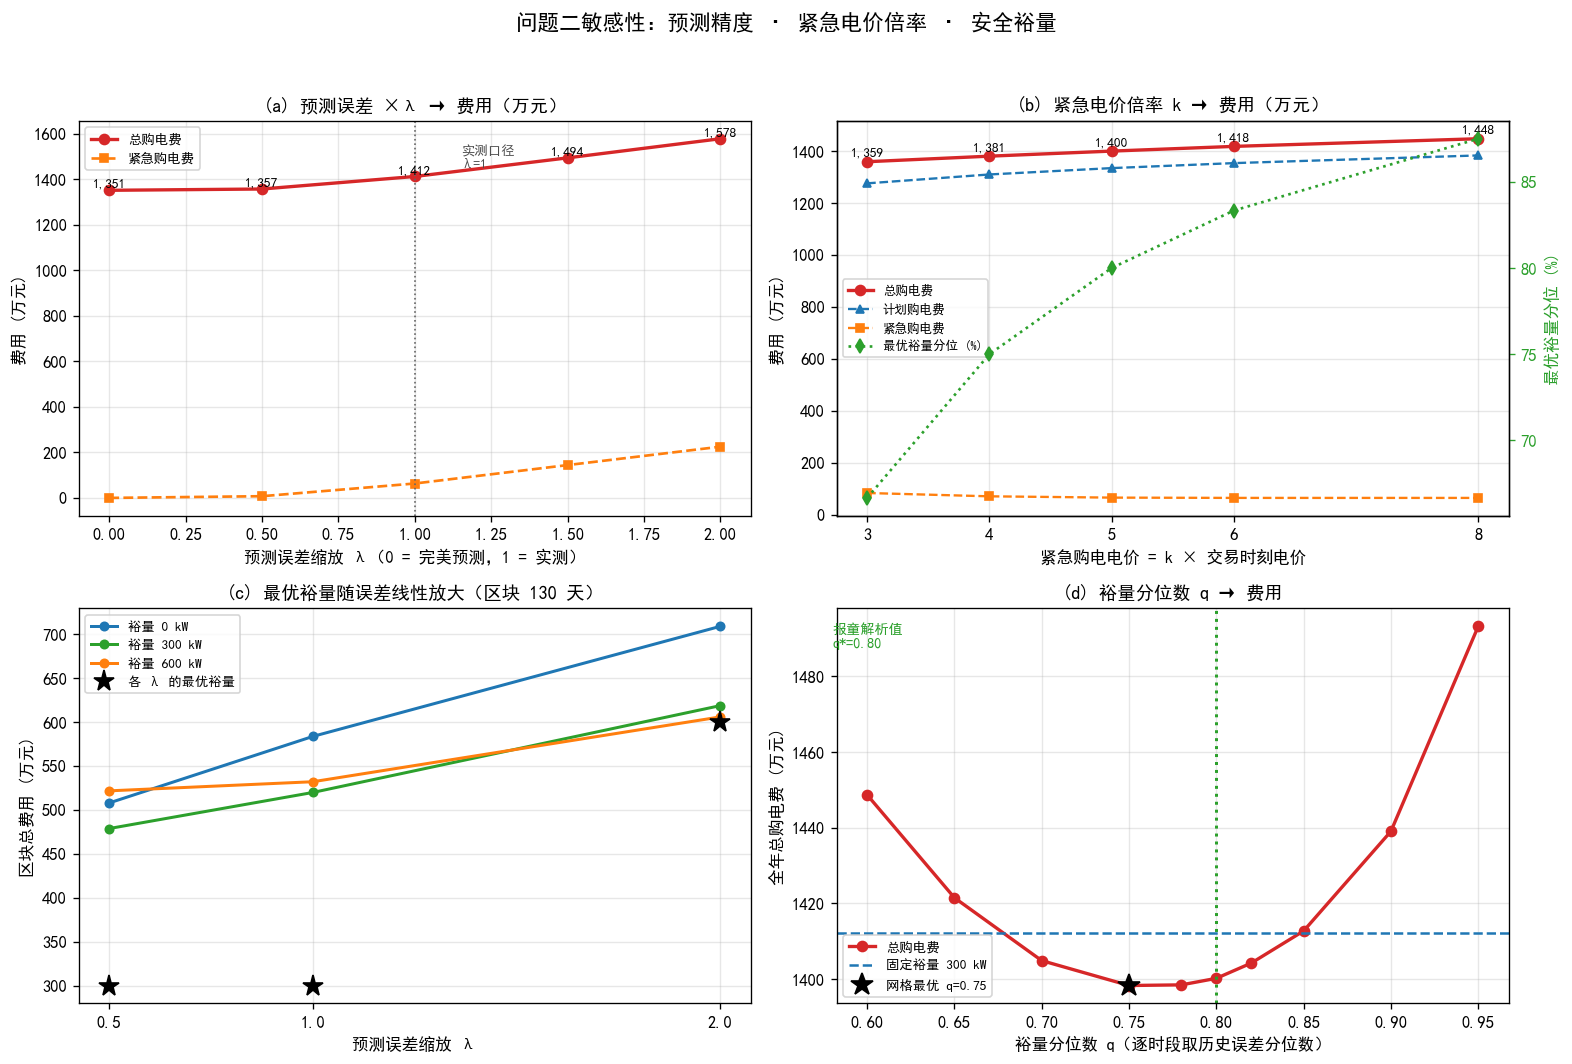
\includegraphics[width=\textwidth]{问题二敏感性分析.png}
\caption{问题二灵敏度分析：(a) 预报误差缩放 $\lambda$ 对总费用与紧急购电费的影响（后者才是增长来源）；(b) 紧急电价倍率 $k$ 与随之变化的最优裕量分位，紧急购电费在 $k\ge6$ 后饱和；(c) 最优裕量随误差幅度同比例放大（报童模型的自检）；(d) 裕量分位 $q$ 的全年费用曲线，谷底平坦且覆盖报童解析值 $q^{*}=0.80$}
\label{fig:q2_sens}
\end{figure}

\subsection{问题三：裕量分位、误差口径与光伏权重}
\begin{enumerate}
    \item \textbf{报童分位数：}$0.70/0.75/0.80$ 三档费用分别为 13\,624\,983.0、13\,589\,362.4、13\,598\,164.7 元，极差 0.26\%，且解析预测区间 $[0.70,0.80]$ 覆盖最优值。
    \item \textbf{裕量误差口径：}负载误差口径与净负荷误差口径的费用差异 $\le0.14\%$（同分位下净负荷口径优 10\,456.6 元），属噪声量级，故保留负载误差口径（见 8.3 节对照实验）。
    \item \textbf{光伏混合权重：}统一权重 $m=0.4$ 与分时段最优权重相比更省 3.8$\sim$6.0 万元；“在最终口径下重扫”得到的最优权重为 0.30，仅比 0.40 省 5\,965.5 元（0.044\%），且把样本切成三段检验时，0.30 只在 1/3 的区段取胜（三段差值 $+2\,034.1$、$+1\,696.2$、$-9\,705.6$ 元），故判定为噪声，保留 0.40。
    \item \textbf{负载自适应限幅：}$\pm20\%$ 使剩余时段 MAE 由 198.4 kW 降至 172.9 kW。
\end{enumerate}

\subsection{问题四：电价波动}
见第 9 节的受控分解：涨价 97.2\% 来自逐日漂移项，窗口内峰谷结构的变化反而使均价略降。

\subsection{一条方法论：预测精度指标与决策目标不等价}
上述所有实验反复出现同一个现象：\textbf{使 MAE 最小的参数，未必使费用最小}。
光伏滑窗的 MAE 最优在 $k_w=5$ 而费用最优在 $k_w=4$；
问题三分时段光伏权重若按 MAE 最优取值，费用反而上升；
问题二的 $\lambda$ 实验更直接——预报精度改善了 4.3\% 的费用，却完全没有改善计划购电费。
根本原因在于\textbf{误差进入费用的方向不对称}：高估光伏会制造缺口并按 5 倍价补电，
低估光伏只是多买了一些本来也需要的电。因此本文所有参数一律以\textbf{全年购电费用}定标，
MAE 仅用于描述预报质量、不作为选参依据。

\section{模型的评价、改进与推广}
\subsection{模型的优点}
\begin{enumerate}
    \item \textbf{统一且自洽的模型族}：问题一至问题四共用同一套约束与执行规则（逐槽被动平衡），保证结果可比较、可复现；问题四仅替换电价输入，形成受控实验。
    \item \textbf{理论有依据的参数}：安全裕量来自报童模型的临界分位数，而非事后试凑；问题三进一步区分两阶段的边际成本结构，给出 $[0.70,0.80]$ 的先验区间，实测最优值正落在其中。
    \item \textbf{精确的 LP 嵌入}：证明并在数值上验证了“逐槽 min/max 规则”可用四组上界约束精确线性化，避免“LP + 仿真”嵌套迭代，全年 334 天四阶段滚动可在数分钟内求解完毕。
    \item \textbf{可量化的下界}：给出完美信息下界 12\,254\,765.7 元，从而把“预报还能带来多少收益”量化为 133.5 万元，为后续投入提供判据。
    \item \textbf{不依赖预测模型的分布假设}：裕量直接取历史误差的经验分位数，避免了正态性等分布假设。
\end{enumerate}

\subsection{模型的不足}
\begin{enumerate}
    \item 报童模型给出的是\textbf{单期}最优分位，而滚动优化是多期耦合（今日多买会改变明日 SOC），严格意义上应使用多阶段随机动态规划；本文用“分位数裕量 + 滚动 LP”近似，实测误差在 0.3\% 量级。
    \item 预测方法仅使用历史统计（周周期 + 滑动平均），未引入数值天气预报（NWP）、云图或温度等外生信息；这既是稳健（不依赖额外数据）也是局限（精度上限受限）。
    \item 购电功率未设上限（见假设 9）。若实际存在联络线容量约束，谷段的大量购电将不可行，需要在模型中增加 $b_t\le B_{\max}$。
    \item 附件 3 的预报只有“整点”点值，本文用线性插值到 10 分钟；若预报本身是小时均值，插值口径应相应改变（会使 MAE 由 191.7 变为 361.6 kW）。
    \item 未考虑储能寿命损耗（充放电次数的折旧成本），因而模型倾向于“高频、深度”使用储能。
\end{enumerate}

\subsection{改进方向}
\begin{enumerate}
    \item 将裕量由“经验分位数”升级为“条件分位数”（如按天气类型、季节分层），可望进一步压缩 133.5 万元的预报误差代价空间。
    \item 引入随机规划或鲁棒优化（如 CVaR 目标），在费用与风险之间显式权衡。
    \item 加入联络线容量、储能循环寿命与需求响应（可平移负载）等约束，使模型更贴近工程实际。
    \item 若可获得多日天气预报，可用第 5 节的自适应修正思路扩展到“多日平滑”，缓解“高负载日恰为高电价日”带来的跨日风险。
\end{enumerate}

\subsection{推广}
本文模型可直接推广到以下场景：含风电/光伏的园区微网日前-日内协调调度；含储能的工商业用户峰谷套利与需量管理；电力市场的日前-实时两结算偏差惩罚问题（问题三的 0.5/1.5 倍价差结构即为典型的两结算机制）；任何“预测误差不对称 + 容量受限”的报童型资源分配问题。

\begin{thebibliography}{9}
\bibitem{ref1} 运筹学教材编写组. 运筹学（第 5 版）[M]. 北京: 清华大学出版社, 2021. （报童模型与临界分位数）
\bibitem{ref2} 陈启鑫, 康重庆, 等. 微电网能量管理与优化调度综述[J]. 电力系统自动化, 2019.
\bibitem{ref3} Mitchell S, O'Sullivan M, Dunning I. PuLP: A Linear Programming Toolkit for Python[R]. 2011.
\bibitem{ref4} Forrest J, Lougee-Heimer R. CBC User Guide[M]. INFORMS Tutorials in Operations Research, 2005.
\end{thebibliography}

\appendix
\section{交付文件与复现方式}
所有程序、中间结果与图表均在交付文件夹内，执行 \texttt{python run\_all.py} 可一键复现全部数值。

\begin{center}
\begin{tabular}{cl}
\hline
文件 & 说明 \\
\hline
\texttt{config.py} & 公共库：数据读取、时间口径、储能仿真、绘图与报告 \\
\texttt{q1.py}, \texttt{storage.py} & 问题一 MILP/LP 与表格填报 \\
\texttt{q2.py} & 问题二两阶段 LP（含报童裕量、逐槽平衡） \\
\texttt{q3.py} & 问题三四阶段滚动 LP（含逐槽规则精确嵌入） \\
\texttt{q4.py} & 问题四：用附件 4 电价重算问题二、三 \\
\texttt{run\_all.py} & 一键复现脚本 \\
\texttt{result1\~{}4*.xlsx} & 交付表格（表1/表2/表3） \\
\texttt{*\_结果汇总.txt} & 各问结果与参数寻优报告 \\
\texttt{q3\_完美信息.txt} & 完全信息下界与分解 \\
\texttt{q3\_嵌入等价性验证.txt} & 逐槽规则 LP 嵌入的等价性验证 \\
\texttt{figures/} & 全部插图 \\
\hline
\end{tabular}
\end{center}

\section{核心代码片段}
\begin{lstlisting}[language=Python]
# 问题三：调整阶段 LP —— 把逐槽被动平衡规则精确嵌入（q3.solve_adjust）
m += pulp.lpSum((1.5*pi[t]*dp[k] - 0.5*pi[t]*dm[k]
                 + 5.0*pi[t]*e[k] + EPS_CUR*s[k]) * DT_H
                for k, t in enumerate(range(t_from, T)))
for k, t in enumerate(range(t_from, T)):
    m += b[k] == b_plan[t] + dp[k] - dm[k]        # 相对计划的偏差
    m += d[k] - c[k] - s[k] - e[k] == Lf[t] - Gf[t] - b[k]
    m += s[k] <= Gf[t]                            # 弃光不超过当时光伏
    prev = E_start if k == 0 else E[k-1]
    m += d[k] <= (prev - SOC_MIN) * ETA / DT_H    # 放电：功率 / 剩余电量
    m += c[k] <= (SOC_MAX - prev) / (ETA * DT_H)  # 充电：功率 / 剩余空间
    m += E[k] == prev + (ETA*c[k] - d[k]/ETA) * DT_H
m.solve(pulp.PULP_CBC_CMD(msg=False))

# 报童分位裕量（q2.build_hedge）：逐时段取历史误差的滚动分位数
X = np.quantile(err[j0:j1, t], q, axis=0) if j1 > j0 else np.zeros(N_SLOT)

# 统一口径的购电量换算（避免把功率直接相加当电量）
q_buy = P_buy * DT_H          # kW * 1/6 h = kWh
total_buy = q_buy.sum()       # 全天购电量 (kWh)
total_cost = (price * q_buy).sum()   # 全天购电费 (元)
\end{lstlisting}

\end{document}
